\documentclass{article}
% Margin definition.
\usepackage[a4paper,total={6.8in, 8.5in}]{geometry}
\usepackage{parskip}
% Images.
\usepackage{graphicx}
\usepackage[hidelinks, bookmarks=true]{hyperref}
\usepackage{float}
% Encoding.
\usepackage[english]{babel}
\usepackage[utf8]{inputenc}
\usepackage{epigraph}
% Allow multiline comments
\usepackage{verbatim} 
% To have another layer of sub sections - \paragraph
\usepackage{titlesec}

\setcounter{secnumdepth}{4}

\titleformat{\paragraph}
{\normalfont\normalsize\bfseries}{\theparagraph}{1em}{}
\titlespacing*{\paragraph}
{0pt}{3.25ex plus 1ex minus .2ex}{1.5ex plus .2ex}
% Helvetic font.
\usepackage[scaled]{helvet}
\renewcommand\familydefault{\sfdefault} 
% Header for UA logo.
\usepackage{fancyhdr}
% package for plots / graphics
\usepackage{pgfplots}
\pgfplotsset{width=10cm,compat=newest}
% Dots in index.
\usepackage[titles]{tocloft}
\renewcommand{\cftsubsecleader}{\Large\cftdotfill{0}}
\renewcommand{\cftsecleader}{\Large\cftdotfill{0}}
\renewcommand{\cftsecfont}{\large\bfseries\scshape}
\renewcommand{\cftsubsecfont}{\scshape}
\renewcommand*{\HyperDestNameFilter}[1]{\jobname-#1}
% Dot after number in (sub)sections and in toc.
\renewcommand{\cftsecaftersnum}{.}
\renewcommand{\cftsubsecaftersnum}{.}
\usepackage{titlesec}
\titlelabel{\hspace{-0.5cm}\quad}
\usepackage[letterspace=45]{microtype}
\newcommand*{\fullref}[1]{\hyperref[{#1}]{\autoref*{#1} \nameref*{#1}}}
% Header with UA logo definition. 
\pagestyle{fancy}
\fancyhf{}
\chead{
    
\includegraphics[width=5in]{./images/header_ua.png}
}
\setlength\headheight{20pt}
% Footer with page number.
\rfoot{Page \thepage}
\renewcommand{\footrulewidth}{0.1pt}
% Rename table of contents title to "Index"
\renewcommand{\contentsname}{\normalsize Index \vspace{0.6cm}}
% Add text with hyperlink
\usepackage{hyperref}
%\hypersetup{
%    colorlinks=true,
%    linkcolor=blue,
%    filecolor=magenta
%}
% Water mark
\newsavebox\mybox
\usepackage[printwatermark]{xwatermark}
\usepackage{xcolor}
\usepackage{tikz}
% paragraph
\newcommand\tab[1][1cm]{\hspace*{#1}}
\setlength\parindent{24pt}
%images
 \usepackage{graphicx}
\usepackage{caption}
% footnotes at bottom
\usepackage[bottom]{footmisc}
% Urls with line break
\usepackage{pdflscape}
% Drawing functions
\usepackage{tikz}
\usepackage{pgfplots}
\pgfplotsset{width=7cm, height=4cm, compat=1.17}

\usepackage{multicol}
\setlength{\columnsep}{1cm}

%%%%%%%%%%%% References/Bibliography %%%%%%%%%%%%
\usepackage{biblatex}
\addbibresource{bibliography.bib}

%%%%%%%%%%%%%%%%%%%%%%%%%%%%%%%%%%%%%%%%%%%%%%%%%

\begin{document}

%%%%%%%%%%%%%%%%%% Cover Page %%%%%%%%%%%%%%%%%%
\title{\vspace{-0.9cm}
       \vspace{1cm}
       \normalsize
       \raggedright\textbf{Title: \hspace{1.5cm} Bitcoin: An Overview} \\ \vspace{0.4cm}
       \raggedright\textbf{Authors: \hspace{0.95cm} Eduardo Santos, Hugo Ferreira, João Soares, Pedro Bastos} \\ \vspace{0.4cm}
       \raggedright\textbf{Date: \hspace{1.45cm} 13/04/2021} \\}
\author{}
\date{}

\maketitle
\thispagestyle{fancy}

%%%%%%%%%%%%%%%%%% END Cover Page %%%%%%%%%%%%%%%%%%

\vspace{-1.4cm}

\tableofcontents


\fontsize{10pt}{13pt}
\selectfont
\lsstyle

\titlelabel{\thetitle.\quad}	

\newpage

\section{Introductory Note}

\tab This report consists of a brief analysis of Bitcoin and its protocol, exploring its surge and growth in the cryptocurrency market, as well as the seven pillars of Bitcoin. The main goals is to explain Bitcoin in a way that anyone can understand.

We will start by addressing the topic of cryptocurrencies, explaining what they, how they work, and how they are compared to the money we know, also going through the topic of cryptocurrencies mining.
We will also address the topic of blockchain, explaining what it is and how does it work.

To finish, we will explain some of Bitcoin's socio-economical impact.

\section{Summary / Abstract}

\tab Cryptocurrencies like Bitcoin have been widely spoken over the past few years, majorly because of what they represent: the beginning of the globalization of digital currencies.

They came as a new way if looking at money, and they wouldn't exit without blockchain.

\section{Cryptocurrency}

\subsection{Definition of Cryptocurrency}

\subsubsection{What is Money}

\tab To understand what is a cryptocurrency, we first need to understand the concept of money as a form of currency, as well as a medium of exchange of goods and services. Before money as we know it existed, the payment/trade of goods and services was made with commodity money.

\paragraph{Commodity Money}
 
\tab Commodity money is a physical good whose value comes from the resource of which it is made, in other words, that has “intrinsic value” - utilization outside of its use as money. As such its underlying value and use ensures that people trust it because it has value in and of itself and so people can trade it freely with the knowledge that someone will accept it. This type of money is usually durable, divisible, easily exchangeable, and rare.

Some historic examples of commodity money being salt (extremely important to conserve food) and tobacco - after World War II some parts of Europe briefly used this type of money.

Eventually, society evolved into a system of representative money and fiat money.

%Added [H] after so that image is placed after the text above
%This is only possible by adding also \usepackage{float} to the preamble
\begin{figure}[H]
    \begin{center}
        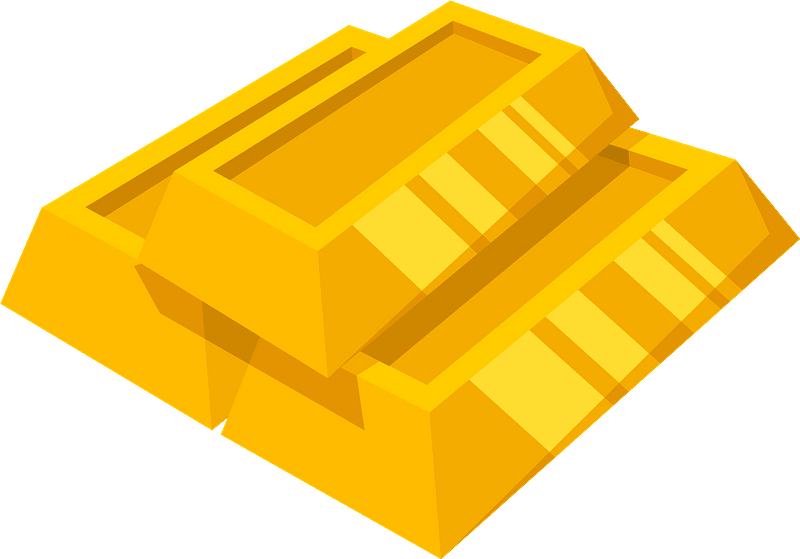
\includegraphics[width=0.2\textwidth]{images/gold.png}
        \caption{\href{https://creazilla-store.fra1.digitaloceanspaces.com/cliparts/60810/gold-bars-clipart-md.png}{\underline{Commodity Money}}}
    \end{center}
\end{figure}

\paragraph{Representative Money}

\tab Representative money is a form of currency often printed on paper that represents something of value - a resource/commodity - but has little or no value of its own. Its acceptance requires that the population trusts the certificate as much as the value that it represents. It was usually backed by a physical resource such as precious metals like gold or silver that existed in the United States as silver certificates or gold certificates issued by state banks. Nowadays, financial instruments like checks and credit cards are the most common forms of representative money.

\begin{figure}[H]
    \begin{center}
        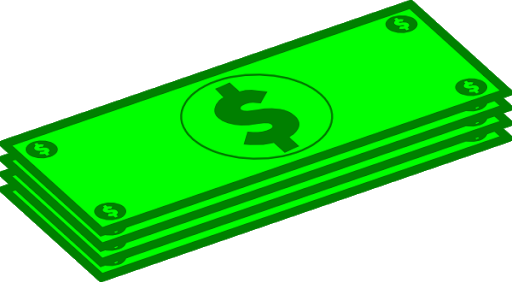
\includegraphics[width=0.2\textwidth]{images/dollar_bills.png}
        \caption{\href{https://lh3.googleusercontent.com/proxy/Kkpz0GitIhYF3RQMX4Rc9adthHDmpJeNtvSA395ZQ8QncVUxUo6ZsF15PNkorqYI5B5XXS18lon4rzLxxtKni9cXvCRebW0}{\underline{Representative Money}}}
    \end{center}
\end{figure}

\paragraph{Fiat Money}

\tab Fiat money is the most common type of currency nowadays, with every other nation operating on some form of fiat money like the Euro or the GBP\footnote{Great British Pound}.

\renewcommand{\epigraphflush}{center}
\epigraph{\textbf{Fiat money is a currency without an underlying value. Instead, its value is derived by government and the trust people place in its value. In other words, it is a form of currency that only holds value because of government enforcement.}}{\textit{Source:\href{https://boycewire.com/fiat-money-definition/#FiatVsRepresentative}{\underline{BoyceWire's definition of fiat money}}}}

It’s a type of money where trust is fundamental because, although its value is given by an official law or order, its true value lies in the trust that people place in it. If consumers and businesses did not trust its enforcement value, then it would not be accepted as a method of payment/trade of goods and services. It is only because people believe others will accept it as a method of payment/trade that it maintains its value, if this did not happened, it would be worthless.

\begin{figure}[H]
    \begin{center}
        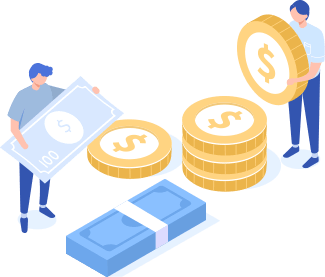
\includegraphics[width=0.3\textwidth]{images/fiat_money.png}
        \caption{\textit{Fiat money}}
    \end{center}
\end{figure}

Some advantages of this type of money is that it can technically be unlimited and it's cheaper to produce, central banks can "print" as much money as they want, and the production cost is small if not null. Because much of the transactions are being done online nowadays.

On the other hand, gold, silver, or any other resource/commodity is limited by the extraction process, for instance on a mine, and the limited nature of its existence with an exorbitant cost, because it requires workers to mine it, process it, transport it, and then finally store it in a safe place.

The two previously mentioned advantages create stability because the money supply can react quicker to an increasing/decreasing economic output and enter the market in a short period of time, preventing and decreasing the effects of cases like the Great Depression by creating a greater level of price stability, in other words controlling high inflation and deflation.

\paragraph{Inflation and Deflation}

Inflation, measured using the consumer price index, is where the price of goods increases over a set period of time, in other words, the price of a good or service is increasing and each unit of currency buys fewer goods and services consequently reflecting a reduction in the purchasing power per unit of money therefore damaging the economy.

Deflation, measured using the consumer price index, is a decrease in the general price level of goods and services, in other words, allows more goods and services to be bought than before with the same amount of currency, being generally associated with a contraction in the money supply. Although it can be positive in the short-term as it can provide a boost to economic growth if consumers believe prices won’t continue to fall, in the long-term, if consumers start to expect deflation every year, they start delaying purchasing decisions in the perspective that they will get the goods and services even cheaper next year which can depress the economic output.

The previously referred stability was demonstrated in the 2008 financial crisis where prices remained relatively stable with inflation rising by an average of over 1,5 percent in the following three years, something that most economists favor while in the Great Depression inflation declined by an average of over 8,8 percent in the following three years.

\begin{figure}[H]
    \begin{center}
        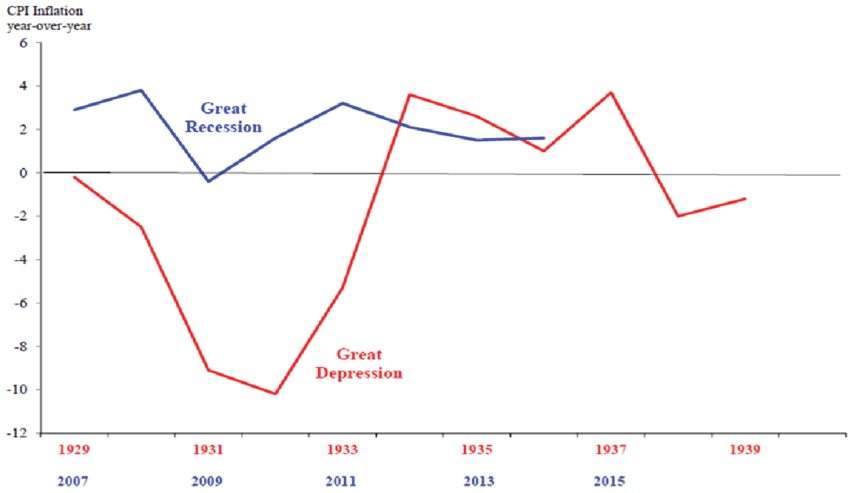
\includegraphics[width=0.6\textwidth]{images/inflation_deflation.png}
        \caption{\href{https://www.researchgate.net/figure/Inflation-and-deflation-rates-during-the-Great-Depression-and-Great-Recession_fig3_321576621}{\underline{Inflation and deflation rates during the Great Depression and Great Recession}}}
    \end{center}
\end{figure}


However, stability relies more on the decisions made by the central banks that can have more of an effect than the type of money or even the type of currency used, as demonstrated by the Venezuela currency, the Bolivar Fuerte, replaced the original Bolivar in 2008, but inflation is still very high because among other factors there are no clear restrictions on how much the government can or cannot print money.

\begin{figure}[H]
    \begin{center}
        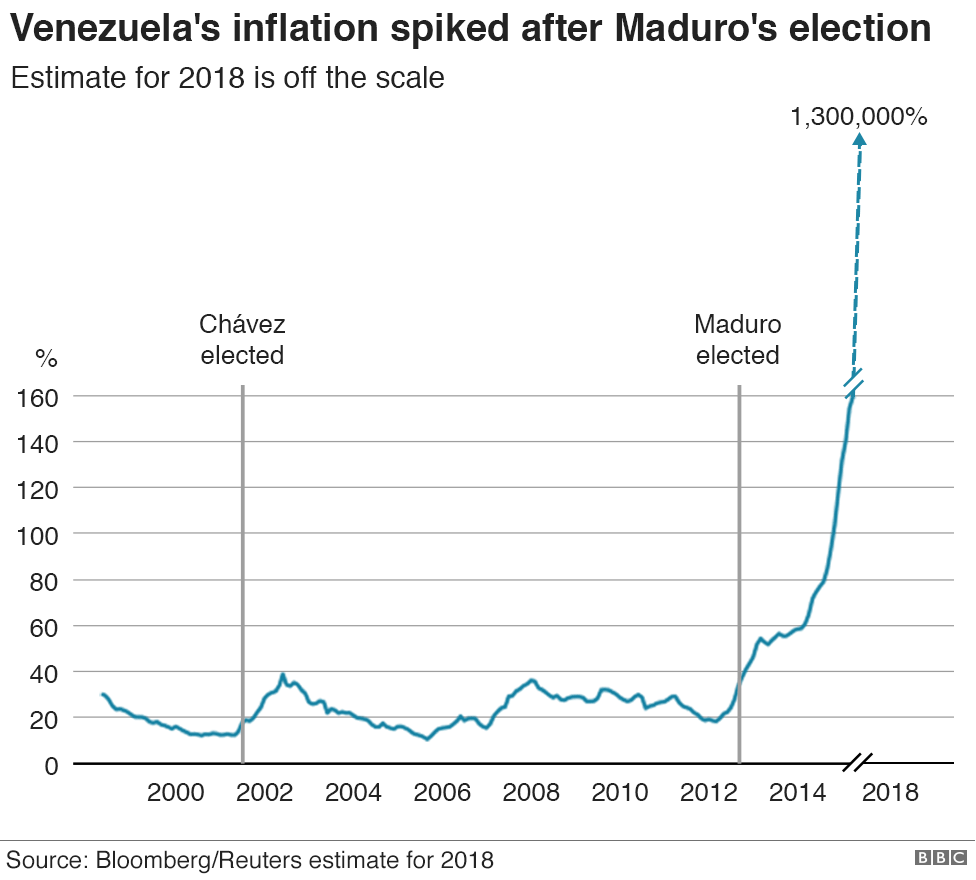
\includegraphics[width=0.5\textwidth]{images/venezuela_inflation.png}
        \caption{\href{https://ichef.bbci.co.uk/news/640/cpsprodpb/7822/production/_105345703_venezuela-inflation_v3_976-nc.png}{\underline{Venezuela's inflation fluctuation between 2000 and 2018}}}
    \end{center}
\end{figure}

\subsubsection{What is Cryptocurrency}

A cryptocurrency is a digital currency, in other words, a medium of exchange that is encrypted and decentralized. Unlike the U.S. Dollar or the Euro, there is no central authority that manages and maintains the value of a cryptocurrency. It doesn't rely on banks to verify transactions, instead it's a P2P\footnote{peer-to-peer} system that can enable anyone anywhere that has a digital wallet to send and receive payments using a technology called blockchain, which we will talk about later on in this report. 

A cryptocurrency wallet doesn't actually hold any currency, it merely provides an address for your funds.

Unlike physical money that is carried around and exchanged, cryptocurrency payments exist purely as digital entries to an online database that describes specific transactions. When you transfer cryptocurrency funds, the transactions are recorded in a public ledger.

It's possible to buy or sell cryptocurrency in exchange for a fiat currency like the U.S. Dollar using a cryptocurrency exchange. Exchanges, which can hold deposits in both fiat and cryptocurrencies, credit and debit the appropriate balances of buyers and sellers in order to complete cryptocurrency transactions. People can also use cryptocurrency to buy  products and services with more and more companies accepting this type of currencies as a payment method.

Cryptocurrency got its name because it uses encryption to provide security and safety in transactions. This means advanced coding is involved in storing and transmitting cryptocurrency data between wallets and to public ledgers. 

\begin{figure}[H]
    \begin{center}
        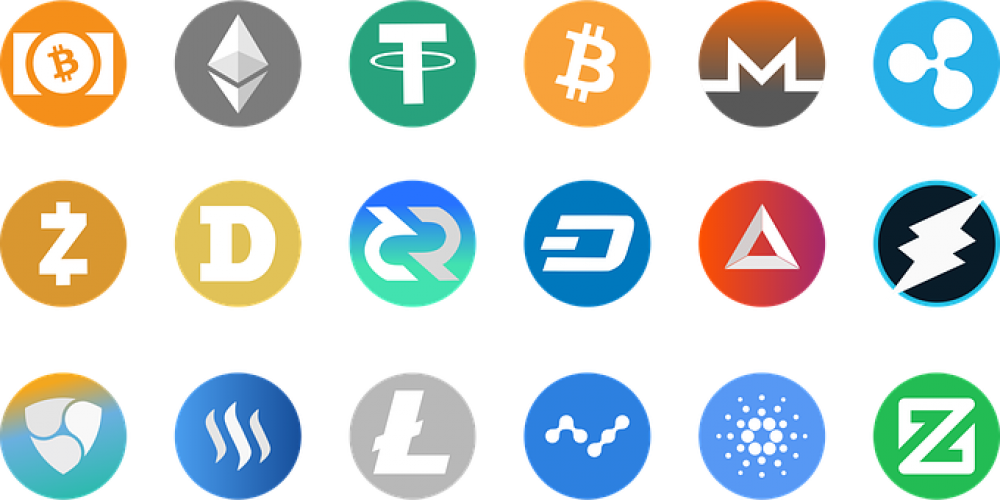
\includegraphics[width=0.5\textwidth]{images/types_of_cryptocurrencies.png}
        \caption{\href{https://coinratecap.com/public/storage/posts/July2019/5aGA2VGhWLCMy27A49my.png}{\underline{Types of cryptocurrencies}}}
    \end{center}
\end{figure}

\subsubsection{Comparison between Cryptocurrencies and Fiat Money}

\tab Compared to fiat money, cryptocurrencies share some characteristics as both can be used for payments and as a store of value. Both rely on widespread trust of people in order to function as a means of exchange although cryptocurrencies' trust and value is based on the underlying technology blockchain while fiat money's value and trust is derived from a governmental institution or a trustworthy authority such as the ECB\footnote{European Central Bank}.

Some key differences are that cryptocurrency is  produced and distributed through a process called mining and most have a cap which means there is a set amount of coins that will ever be in supply, making it possible to tell the amount in circulation at any given time, something impossible in fiat money.
 
Cryptocurrency is not controlled by a centralised authority, transactions can’t be reversed, cancelled or charged back and while fiat money can be physical, cryptocurrency is only digital.

\begin{figure}[H]
    \begin{center}
        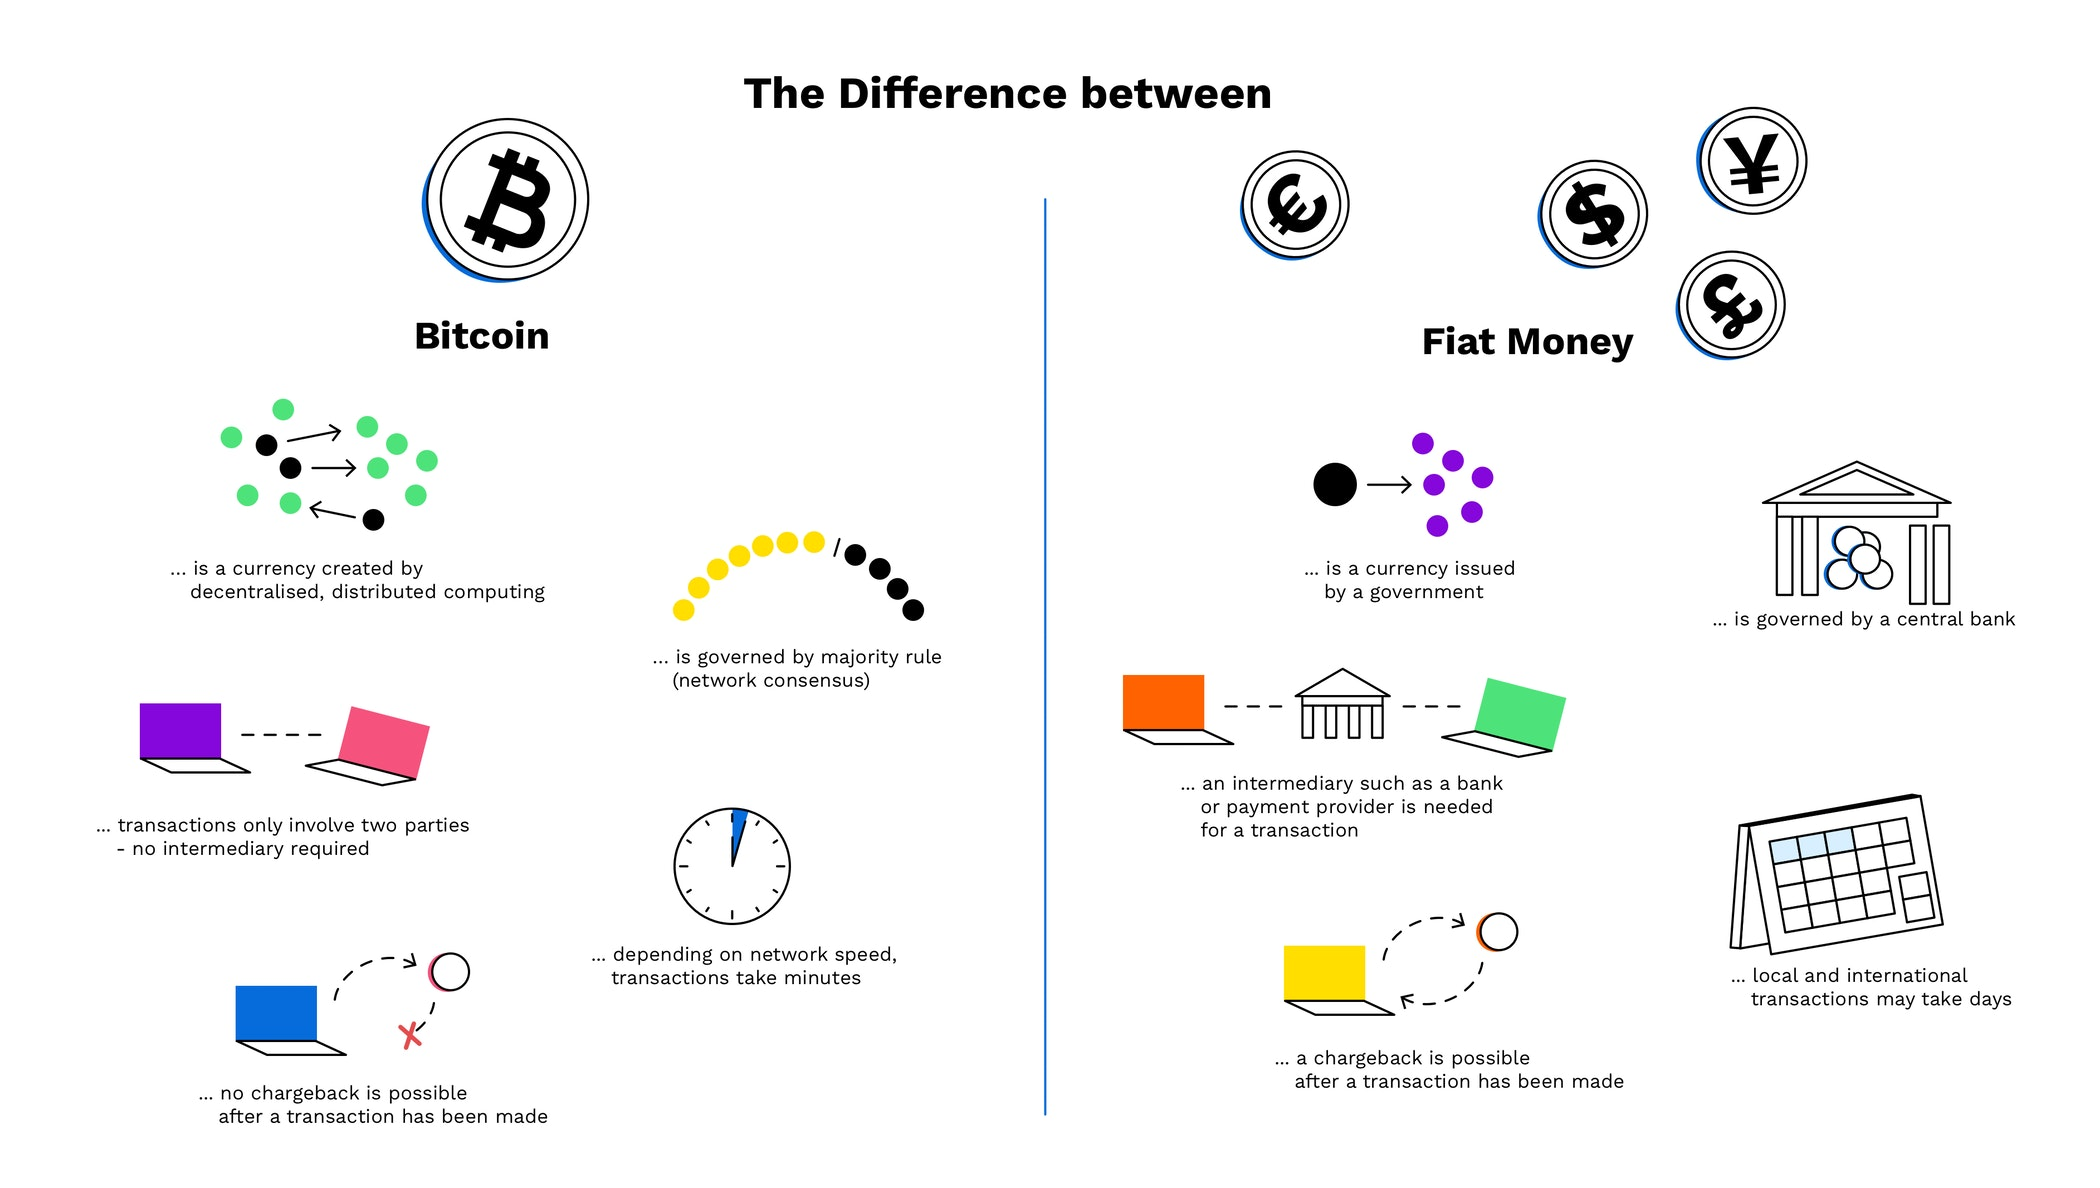
\includegraphics[width=0.8\textwidth]{images/cryptocurrencies_vs_fiat_money.jpeg}
        \caption{\href{https://bitpanda-academy.imgix.net/null94a7b99f-2399-48fa-a503-876e2ba6f2bf/Bitpanda-Infographics_2-bitcoin_fiat.png?auto=compress\%2Cformat&fit=min&fm=jpg&q=80&w=2100}{\underline{Difference between cryptocurrencies and fiat money}}}
    \end{center}
\end{figure}

\subsection{How Cryptocurrencies Work}

\tab Cryptocurrencies work using a technology called blockchain. Blockchain is a decentralized technology spread across many computers that manages and records transactions in a way that makes it difficult or impossible to change, hack, or cheat the system, a characteristic that constitutes much of the appeal for this technology.

We will talk more about blockchain on the next section.

\subsection{Cryptocurrrencies Mining}

\tab The process by which new currency is produced and entered into circulation is designated as Mining. Mining is also a critical process of the maintenance and development of the blockchain ledger is performed by high power computers that require either a GPU\footnote{Graphics Processing Unit} or an ASIC\footnote{Application-Specific Integrated Circuit} in order to set up a mining rig, to solve complex computational math problems. When computers solve these complex math problems on the network, they produce new cryptocurrency (similar  when a mining operation extracts gold from the ground) and by solving the computational math problems, miners make the blockchain network trustworthy and secure by verifying its transaction information. 

Transactions made in-store or online are documented by Banks, point-of-sale systems, and physical receipts and Miners achieve the same by clumping transactions together in blocks and adding them to the blockchain. When Miners add a new block of transactions to the blockchain, they need to make sure that those transactions are accurate. In particular, make sure that the cryptocurrency is not being duplicated, a characteristic of  digital currencies designated as “double-spending.”

Miners after completing blocks of verified transactions which are added to the blockchain can then receive a reward if they are the miner who discovers a solution to a complex computational math problem first, and the probability that a Miner will be the one to discover the solution, is related to the portion of the total mining power on the network making mining a very meticulous, costly, and only sporadically rewarding but nevertheless important.

\begin{figure}[H]
    \begin{center}
        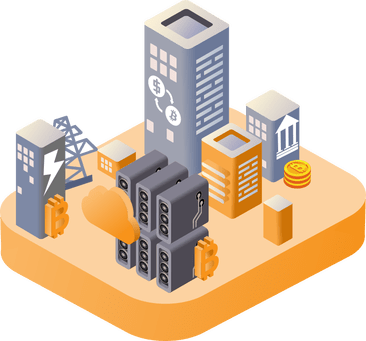
\includegraphics[width=0.3\textwidth]{images/bitcoin_mining.png}
        \caption{\href{https://miro.medium.com/max/366/0*hSBQbC__jrcu2jeg}{\underline{Bitcoin Mining}}}
    \end{center}
\end{figure}

As previously mentioned, to make transactions in cryptocurrency, you need a wallet for that currency, that in fact doesn't hold any currency as it merely provides an address for your funds on the blockchain. A cryptocurrency wallet also includes private and public keys that enable you to complete secure transactions.

So every time it's made a transaction to payment of goods and services or transfer cryptocurrency, an individual authorizes the movement of a specified amount of the cryptocurrency from his wallet address to the wallet address of the seller. The transaction is encrypted with the individual private key and pushed to the blockchain. The cryptocurrency network's miners access the individual public key to confirm that his private key was used to encrypt the transaction. Once the block that includes the individual transaction is confirmed, the ledger is updated to show the new cryptocurrency balances for both the individual address and the seller's address and the miner may be rewarded with cryptocurrency for confirming the transaction, with this entire process being conducted by software.

\section{Blockchain}

\subsection{What is the blockchain}

\tab A blockchain is a chain of blocks that contains information. A blockchain is a distributed ledger that is completely open to anyone, and it relies on a key property: when some data is recorded inside a blockchain, it becomes very difficult to change it. But how does that work?

Each block in the blockchain contains:

\begin{itemize}
    \item \textbf{Data} - this stored data depends on the type of blockchain. In the case of the Bitcoin blockchain, it stores the following details:
    \begin{itemize}
        \item Sender
        \item Receiver
        \item Amount of coins to be traded
    \end{itemize}
    \item \textbf{Hash of the block} - it works like a fingerprint, identifying the block and all of its contents and it is always unique.
    \item \textbf{Hash of the previous block} - this creates a chain of blocks, they form the blockchain itself.
\end{itemize}

Once each block is created, its hash is calculated. Changing something inside the block, will cause the hash to change. In another words, hashes are very useful when we want to detect changes to blocks, if the fingerprint of a block changes, it no longer is the same block.

\subsection{How does it work?}

\tab Let's take, for instance, the chain of blocks in the image below:

\begin{figure}[H]
    \begin{center}
        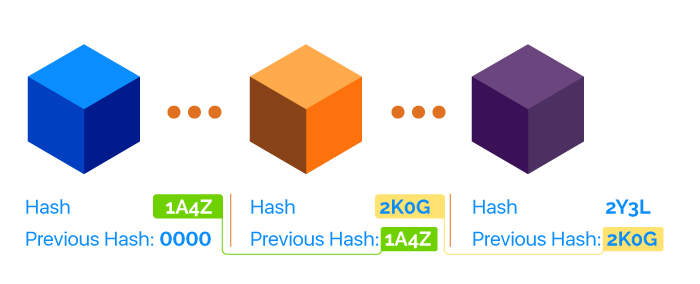
\includegraphics[width=0.6\textwidth]{images/changes_in_block.png}
        \caption{\textit{Example of a blockchain}}
    \end{center}
\end{figure}

As we can see, each block has a hash and the hash of the previous block. So block number 2 points to block number 1, and block number 3 points to block number 2. The first block is called the \textit{Genesis Block}, as it has not got previous blocks.

Now, let's say that someone tampers with the second block, as shown in the image below:

\begin{figure}[H]
    \begin{center}
        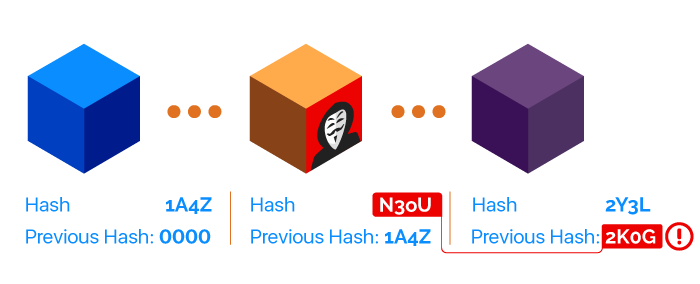
\includegraphics[width=0.6\textwidth]{images/invalid_hash.png}
        \caption{\textit{Example of a tampered blockchain}}
    \end{center}
\end{figure}

This will cause the hash of the block to change as well. This change will make block 3 and all following blocks invalid because they no longer store a valid hash of the previous block. So changing a a single block will make all following blocks invalid.

But using hashes is not enough to prevent tampering. Computers these days are very fast and can calculate hundreds of thousands of hashes per second, this being said, we could tamper with a block, and recalculate all the hashes of the previous blocks to make our blockchain valid again.

To mitigate this, blockchains have something called proof-of-work.

\subsubsection{Proof-of-work}

\tab Proof-of-work is a mechanism that slows down the creation of new blocks. In Bitcoin's case, it takes about ten minutes to calculate the required proof-of-work and add a new block to the chain. This mechanism makes it very hard to tamper with the blocks, because if we tamper with one block, we will need to recalculate the proof-of-work for all the following blocks.

So, the security of a blockchain comes from its creative use hashing and the proof-of-work mechanism.

But there is one more way that blockchains secure themselves, and that is by being distributed. Instead of using a central entity to manage the chain, blockchains use a P2P network that anyone can join. When someone joins this network, he gets the full copy of the blockchain, the node can use this to verify that everything is still in order.

But what specifically happens when someone creates a new block? That block is sent to everyone on the network, each node then verifies the block, to make sure that it has not been tampered with. If everything checks out, each node adds this block to their own blockchain. 

All the nodes in this network create consensus: they agree about what blocks are valid and which are not. Blocks that are tampered with will be rejected by other nodes in the network. This being said, to successfully tamper with a blockchain we would need to tamper with all blocks on the chain, redo the proof-of-work for each block, and take control of more than 50\% of the P2P network. Only then our tampered block would be accepted by everyone else. This entire process is almost impossible to do!

\subsubsection{Smart contracts}

\tab Blockchains are also constantly evolving. One of the most recently developments is the creation of smart contracts.

These contracts are simple programs that are stored on the blockchain and can be used to automatically exchange coins, based on certain conditions.

\section{Bitcoin}

\subsection{What is Bitcoin}

\tab As its name suggests, Bitcoin is an electronic currency, but unlike government issued currencies, there is no single entity that issues Bitcoin or is in charge of processing its transactions. 

Before Bitcoin, it was not possible to make electronic payments without the help of a third party, like a bank or payment processor. Payments were often slow, expensive, and not available to everyone. To solve those problems, Bitcoin operates without a trusted third party, instead, it works as a P2P electronic currency, meaning that payments are sent directly from one person to another.

That works by simply putting computers all over the world, using mathematical functions to independently verify all Bitcoin transactions, which are then added to a public a blockchain, which we already know it works.

Early on in Bitcoin's history, there are very few transactions being processed by the network, but as time went on, more and more people started using this cryptocurrency, so the number of transactions to be processed went up too. Eventually, the Bitcoin network needed to be updated, to keep transactions fast, cheap, and reliable. But, because there was not consensus on how this update should be performed, or wether it should be implemented at all, Bitcoin ultimately had to split into two separate currencies for that update to happen:

\begin{itemize}
    \item \textbf{Bitcoin Cash (BCH)} - this was the version that implemented the original planned update. Bitcoin Cash can currently process over one hundred transactions per second, with fees reliably less than a 0.01 USD per transaction.
    \item \textbf{Bitcoin (BTC)} - this version made different updates to the network, and kept the original name and symbol. Bitcoin can only process between 3-7 transactions per second, and is now considered by many to be digital gold, instead of digital cash. Its fees have ranged anywhere from several cents to tens of dollars per transaction, depending on the number of people trying to use the network at once.
\end{itemize}

\begin{figure}[H]
    \begin{center}
        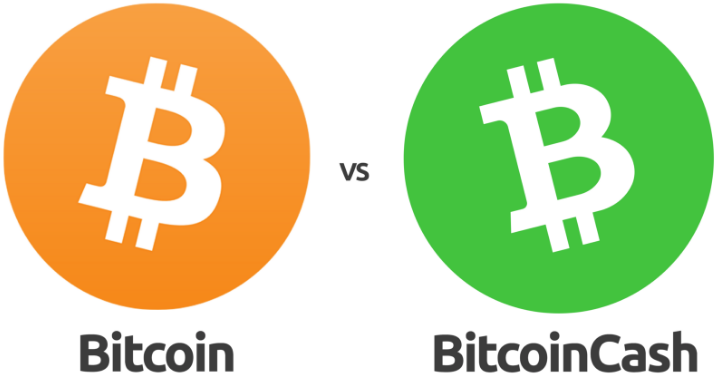
\includegraphics[width=0.4\textwidth]{images/bitcoin_vs_bitcoin_cash.png}
        \caption{\href{https://cdn-images-1.medium.com/max/719/1*kW1BN8Zq8YGR1YYYK2kv9g.png}{\underline{Bitcoin vs Bitcoin Cash}}}
    \end{center}
\end{figure}

\subsection{The Pillars of Bitcoin}

\tab The Bitcoin system has seven main pillars that allow the construction of a fair market. 

\begin{figure}[H]
    \begin{center}
        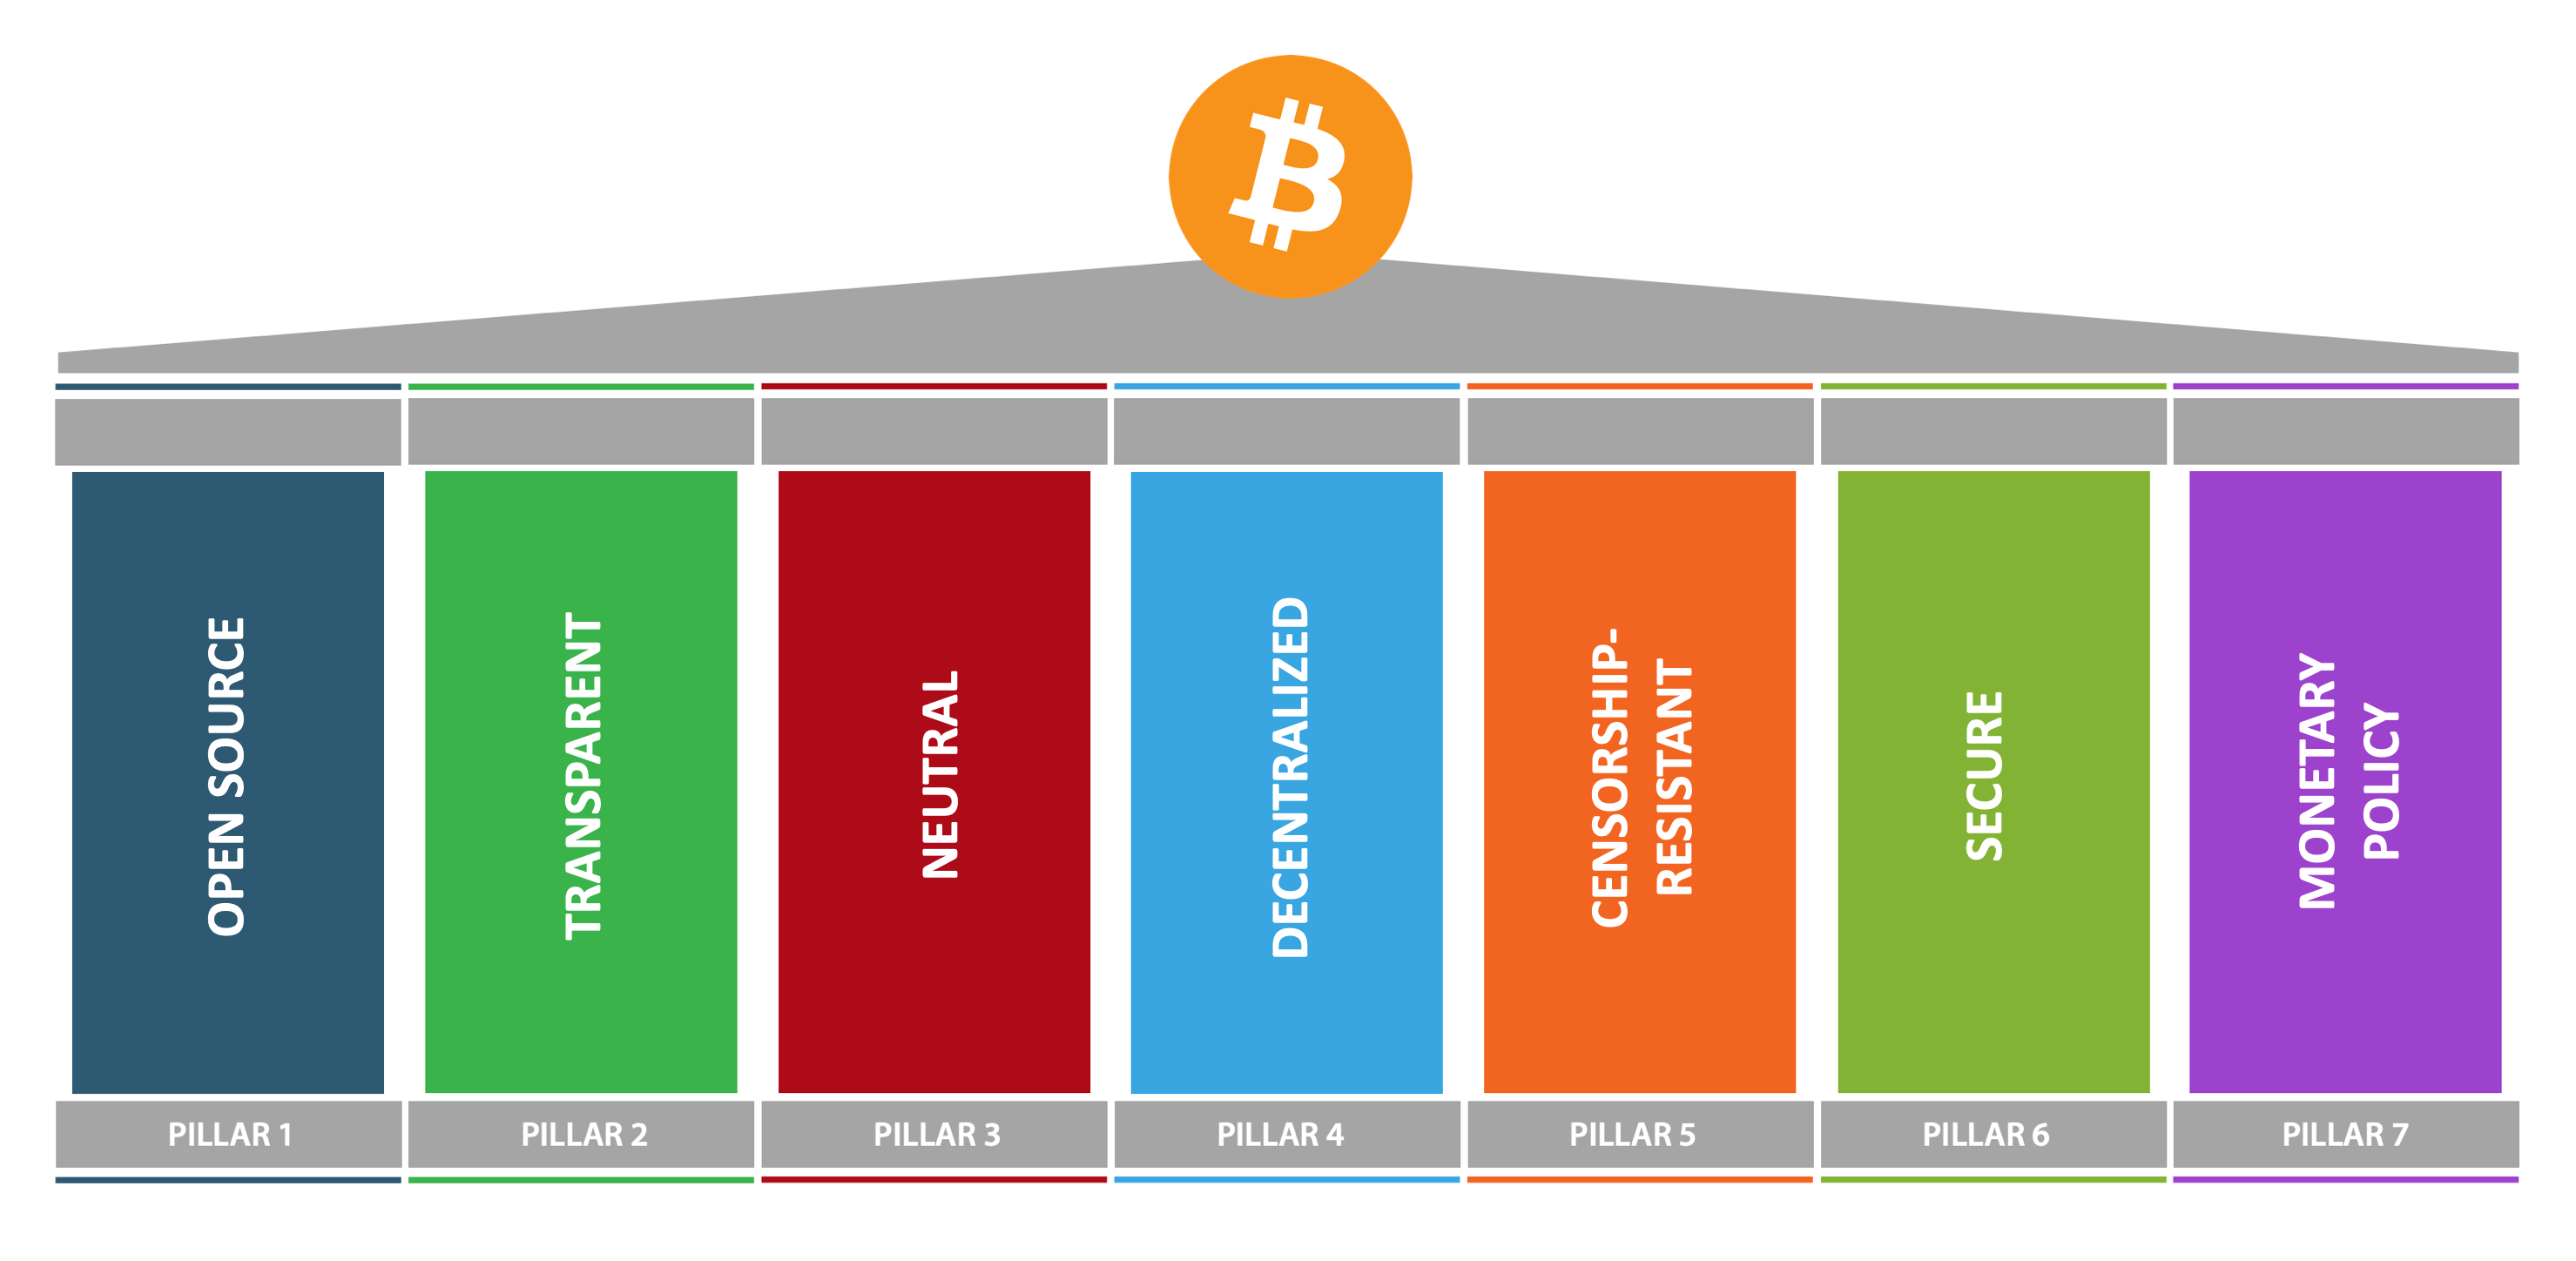
\includegraphics[width=0.6\textwidth]{images/pillars.png}
        \caption{\textit{Pillars of Bitcoin}}
    \end{center}
\end{figure}

\subsubsection{Open Source}

\tab This will be the first pillar approached. Bitcoin is based on the open source software core. This means that the source code is available to anyone who wants to see how the network works. Not only that, anyone can contribute to it. There is a resemblance with the Linux community. The community that daily keeps improving it is its main strength.

With that in mind, bitcoin will not be replaced by a more powerful technology. As mentioned earlier, its developers will keep improving it, making it evolving alongside the internet. Besides that, its security is an essential point to keep improving. And again, thanks to its developers, it will keep up, allowing bitcoin to continue its dominance in the cryptocurrencies market.

\subsubsection{Transparent}

\tab As it was explained in the open source topic, bitcoin blockchain is based on open source code and anyone can check it. Besides that, anyone can enter the network, making bitcoin trustless and permissionless. Anyone can verify any transaction made in the network. This allows people to form their own opinion regarding this market. That is why bitcoin is originally based on a simple quote:

\renewcommand{\epigraphflush}{center}
\epigraph{\textbf{Don't trust, verify.}}{\textit{Bitcoin's motto}}

This is a very important aspect of bitcoin. All users can verify everything by their own, making their decisions a lot easier and allowing them the opportunity to see the impact of every transaction.

\subsubsection{Neutral}

\tab As this system, capable of revolutionizing the current financial system, is available to literally anyone, the success of bitcoin its every user's responsibility. And by this we mean that the users are the ones who make the difference. So, there isn't really an owner of bitcoin. Everyone has equally the same influence. With this, your transactions are only made by you and no one can have a say in it. 

There are many studies that point bitcoin to the U.S dollar's next replacement as the world's reserve currency. They predict the fall of the U.S dollar and the rise of bitcoin, as it is politically neutral. 

\subsubsection{Decentralized}

\tab The whole bitcoin system is decentralized. This means that it is distributed and resistant to potential attacks. Because of this, its up-time is incredibly high: \textbf{99.985\%}, making it almost unbreakable. 

Bitcoin remains the easiest, fastest and most efficient solution to transfer any amount of money across the world. When compared to other solutions, like banks, its transaction fees and taxes are almost insignificant. In addition, the transaction time is also much faster, completing any transaction in 10 minutes. This is usually 300 times faster than any bank transaction. 

As you probably go to this, it is pretty obvious that bitcoin allows you to make transactions without the inter bank system making it difficult.

\subsubsection{Censorship-Resistant}

\tab As we discussed before, bitcoin has always been a democracy in the sense that there is no leader, all users are equally relevant. Each users possesses their own bitcoins as long as they have their private keys, and no one can take that away. 

\renewcommand{\epigraphflush}{center}
\epigraph{\textbf{Not your keys, not your Bitcoins.}}{\textit{Bitcoin's rules}}

Therefore, you have no fear that your bitcoins will be confiscated by any government. This is a major guarantee that you can have by owning bitcoins.

\subsubsection{Secure}

\tab Bitcoin miners are responsible for validating blocks of transactions by allowing their own computing power to be used by the network. To ensure that these miners run the operation smoothly, they are rewarded by 2 things:

\begin{itemize}
    \item \textbf{Halving - Bitcoin reward every 210,000 blocks issued}
    \item \textbf{Transaction fees}
\end{itemize}

 Currently, this makes bitcoin the most secure network in the entire world. 
 
\subsubsection{Monetary Policy}

\tab The bitcoin's policy will prevent bitcoin from its vanishment. Unlike the U.S dollar, bitcoin exists in limited amounts, as there will be no more than 21 million BTC\footnote{Bitcoins} in circulation. This ensures users that they always own the same percentage of the world's bitcoins as time goes by.

In addition, the process of creating new bitcoins is always predictable. No one can change it and everyone can know when new bitcoin will be created, as it is not influenced by any human decision. 

This makes bitcoin's policy better than the one practiced by the banks. The banks' policies change the money quantity and this is not a problem with bitcoin.

\subsubsection{Media}

\tab This one is not a main pillar, its more of a support one. As in almost everything, the press and social media have a huge impact and can almost "move mountains" and Bitcoin has not overlooked this phenomenon, having had great success and appreciation thanks to it.

It all started on a small forum (at the time), Bitcoin Talk, where Laszlo Hanyecz posted a potential Bitcoin transaction for two Papa John’s pizzas that were bought for 10,000 Bitcoins, worth millions today. This simple social forum transaction has led to bigger things, and thus began the interest of social media and press in Bitcoin.

In fact Bitcoin can attribute much of its growth to social forum Reddit where crypto-enthusiasts to crypto-analysts and even crypto-journalists got the most updated Bitcoin news and stories and had and still have detailed information on everything about Bitcoin. This started the construction of the Trust that today people have in cryptocurrencies with for instance most of the trending cryptocurrency stories that hit other social media networks  having origins in Reddit.

A more recent example of this social media impact was when billionaire Elon Musk changed his Twitter bio to include “#bitcoin” which made it climb on the market 15\%.

\begin{figure}[H]
    \begin{center}
        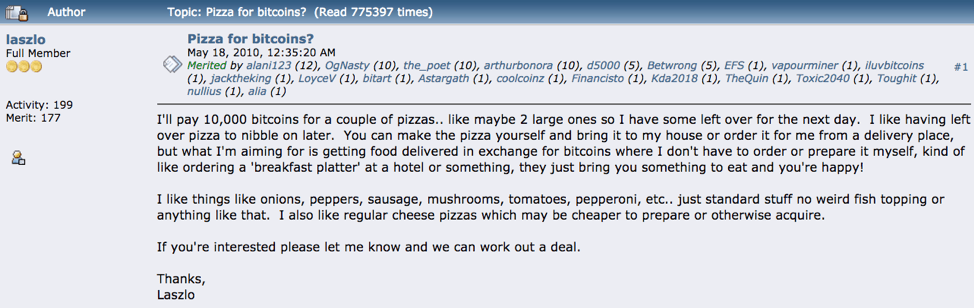
\includegraphics[width=0.8\textwidth]{images/pizzas.png}
        \caption{Pizza for Bitcoins}
    \end{center}
\end{figure}


\subsection{The Bitcoin Protocol}

\tab Being a decentralized digital currency, Bitcoin is not something that we can physically own, which in itself generates a large deviation from the concept of money that we are used to and that we use in our day-to-day. To use this digital asset, there are many steps/rules that need to be followed, they make up the Bitcoin protocol.

Bitcoins are not stored centrally nor locally, they exist in a distributed ledger called blockchain. This ledger runs on a P2P network of computers. 

Owning a Bitcoin is, nothing more, nothing less than simply having the power to transfer it to someone else, with the transaction being recorded in the blockchain. But how does this work?

This is made possible with the usage of an private key - public key ECDSA\footnote{Elliptic Curve Digital Signature Algorithm} pair.

\subsubsection{ECDSA}

\tab ECDSA is a variant of the DSA\footnote{Digital Signature Algorithm}, this uses elliptic curve cryptography. An elliptic curve is mathematically represented by the following equation:

\[y^2 = ax^3 + bx + c\]

In the case of Bitcoin:

\[a = 1\]
\[b = 0\]
\[c = d\: mod\: p\]
\[d = 7\]
\[p = 1.158 \times 10^{77}\]

Replacing the values, we obtain:

\[y^2 = x^3 + 7 \bmod{1.158 \times 10^{77}}\]

Finally, this equation can be translated to the following graphic:

%\vspace{5mm} %5mm vertical space

%Added [H] after so that image is placed after the text above
%This is only possible by adding also \usepackage{float} to the preamble
\begin{figure}[H]
    \begin{center}
        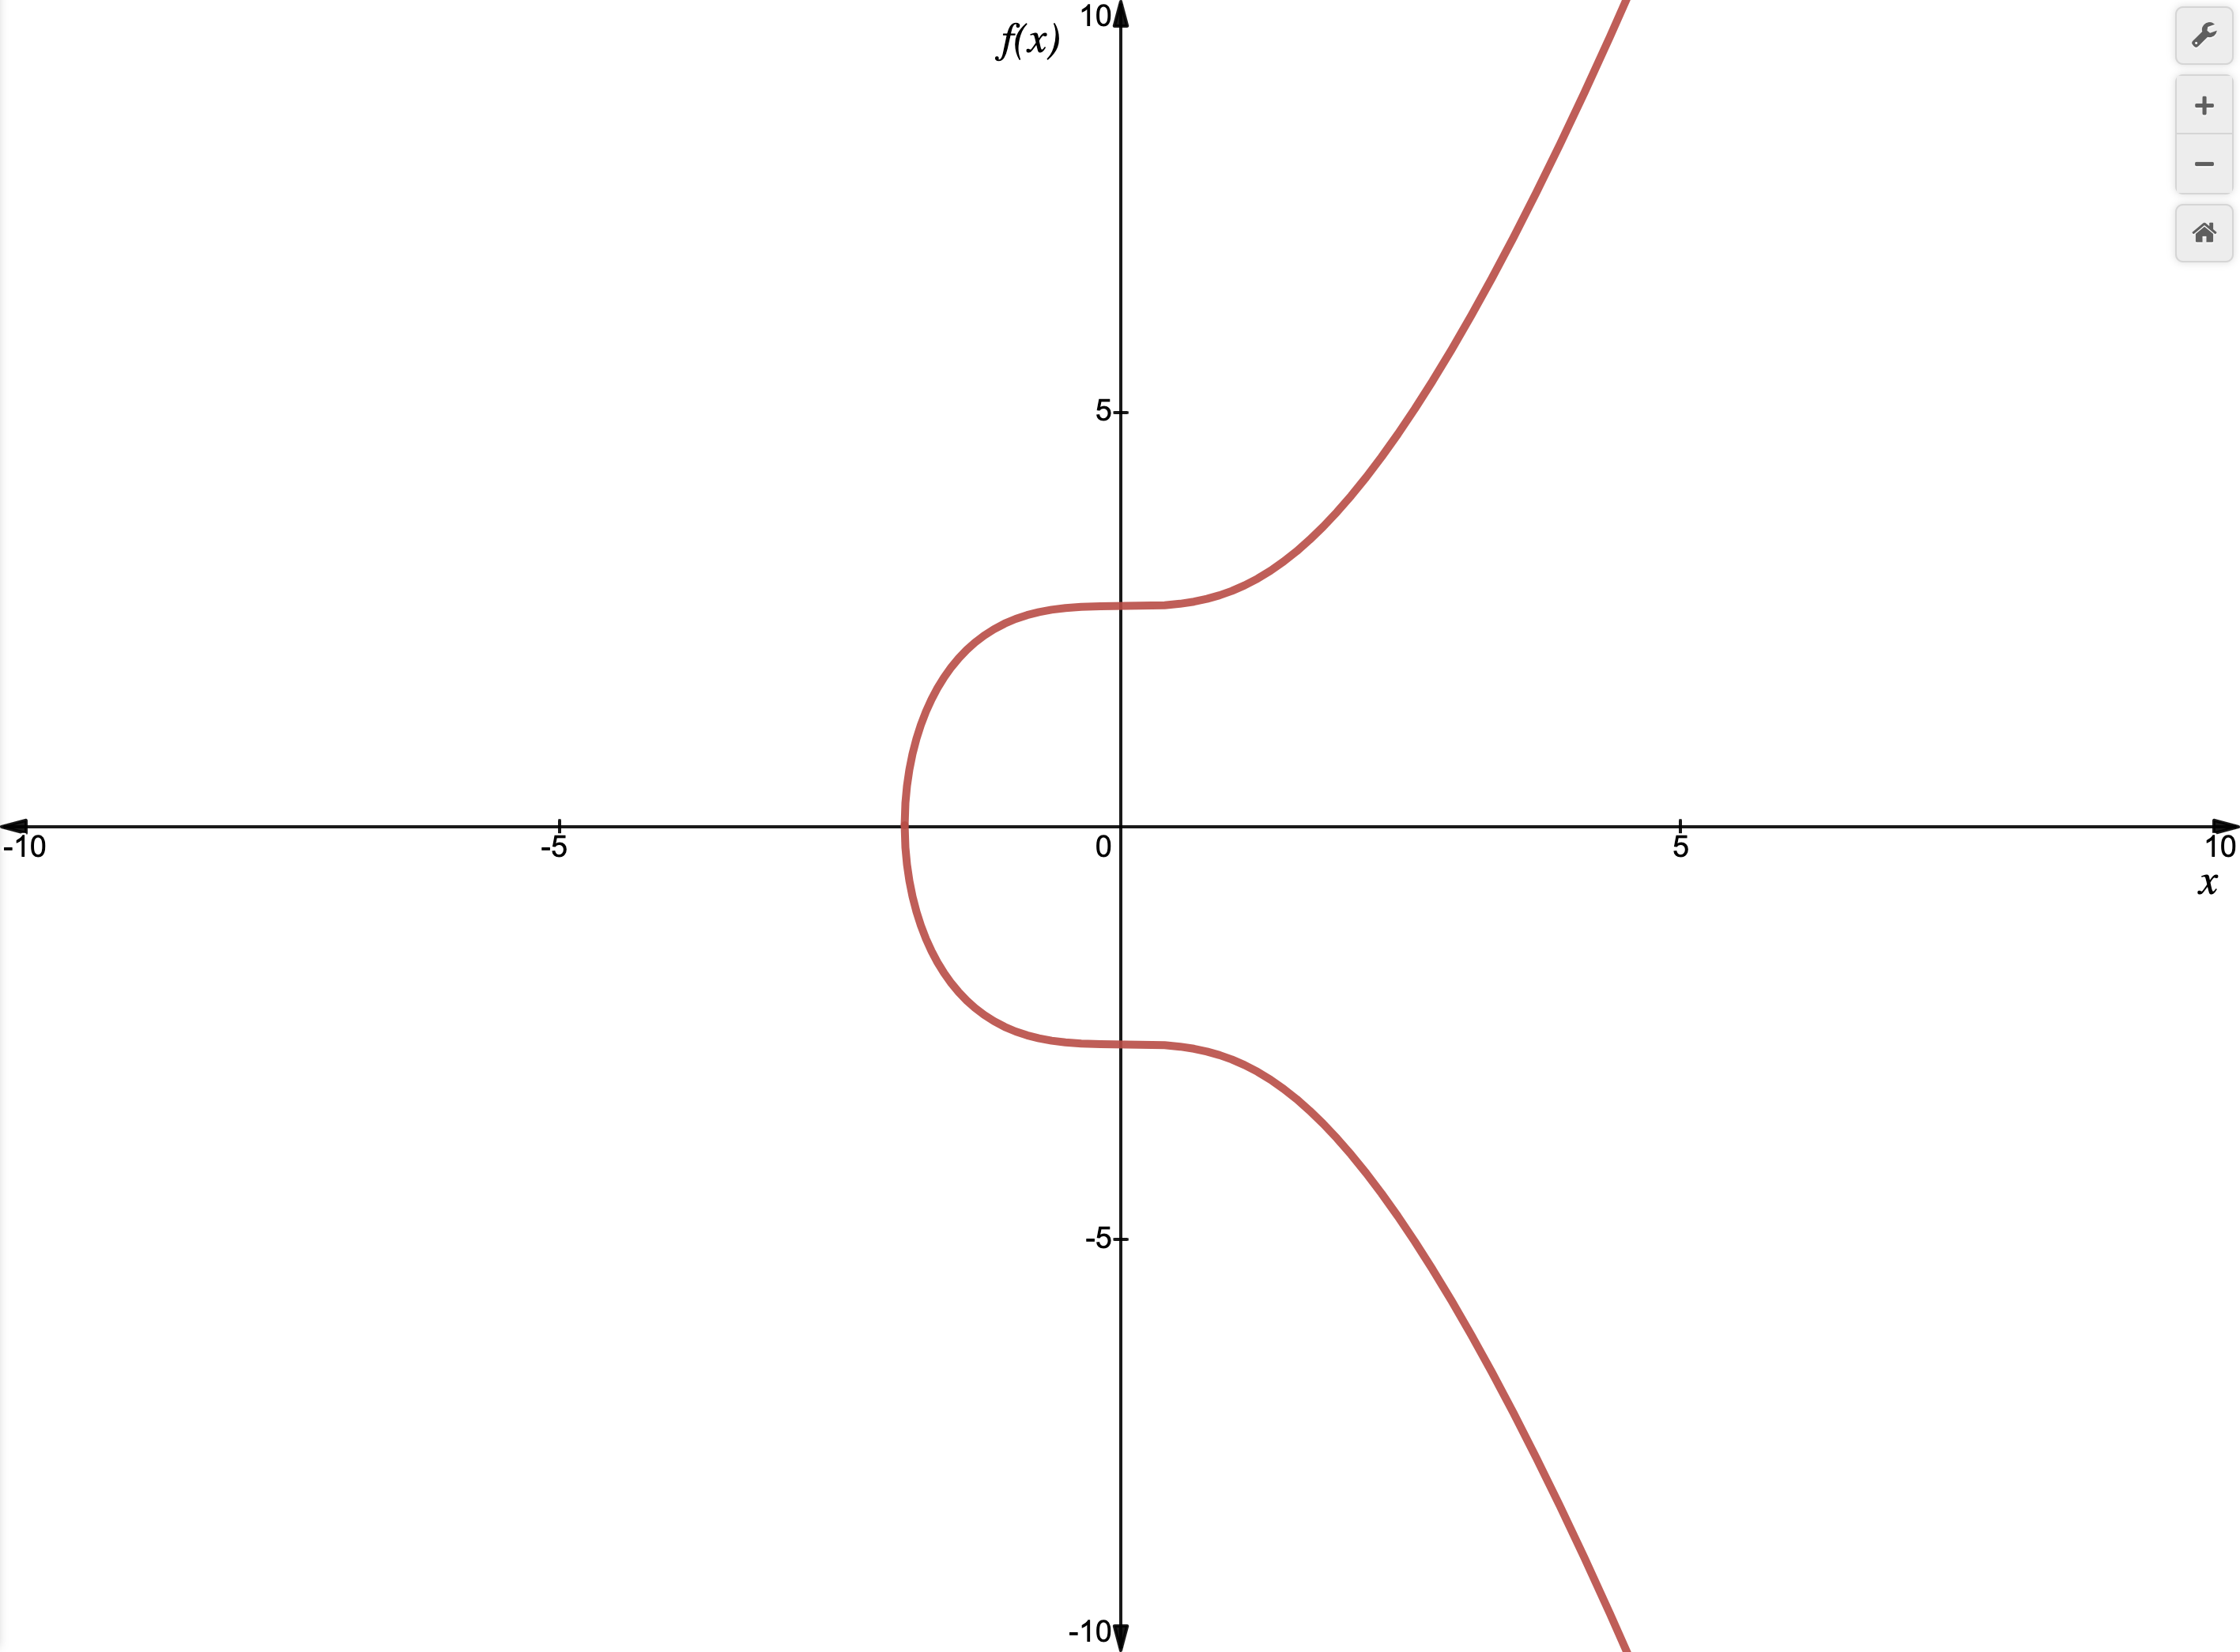
\includegraphics[width=0.5 \textwidth]{images/Kobiltz_curve.png}
        \caption{\textit{Kobiltz curve}}
    \end{center}
\end{figure}

%\vspace{5mm} %5mm vertical space

\begin{comment}
%Added [H] after so that image is placed after the text above
%This is only possible by adding also \usepackage{float} to the preamble
\begin{figure}[H]
    \begin{center}
        \begin{tikzpicture}
            \begin{axis}[
                width=0.5\textwidth,
                height=0.3\textwidth,
                xmin=-5,
                xmax=5,
                ymin=-5,
                ymax=5,
                xlabel={$x$},
                ylabel={$f(x)$},
                scale only axis,
                axis lines=middle,
                smooth,
                domain=-1.912931:3, %supostamente, sem esta linha o gráfico divide-se em 2 partes
                xtick={-5,...,0,...,5},
                ytick={-5,...,0,...,5},
            ]
                \addplot [red] {sqrt(x^3 + mod(7, 1.158*10^(77)))};
                \addplot [red] {-sqrt(x^3 + mod(7, 1.158*10^(77)))};
            \end{axis}
        \end{tikzpicture}
    \end{center}
    \caption{Kobiltz curve}
\end{figure}
\end{comment}

The curve on the graph above is called \textit{Kobiltz curve}, and its often referred as \textit{secp256k1}. This curve was created on purpose, and with a very defined objective: to increase efficiency in the generation of public and private keys, making the computation of this key pair 30\% faster. But this is not the only thing that differentiates this curve from the rest of the elliptical curves, due to the precision in choosing the values of the constants \(a, b, c\) and \(d\), the probability of having an attack in the process in a way that can compromise it is as small as possible.

Elliptic curves have some properties, in  this case, for example:

\begin{itemize}
    \item A non-vertical line that intersects two non-tangent points on the curve will always intersect a third point on the same curve.
    \item A non-vertical line tangent to the curve at one point will intersect only one other point on the curve.
\end{itemize}

This properties allow us to define two operations: point addition and point doubling.

\paragraph{Point addition}

\tab Point addition consists of following this steps:

\begin{itemize}
    \item Take two points of the elliptic curve, \(P\) and \(Q\).
    \item Pass a line through the previous points.
    \item Mark the point (\(-R\)) from the intersection of the previous line with the curve.
    \item Mirror \(-R\) through the x-axis, obtaining \(R\).
\end{itemize}

This algorithm can be put into the following expression:

\[P + Q = R\]

With \(R\) being the result of the sum of the original points.

Finally, this equation can be translated to the following graphic:

\begin{figure}[H]
    \begin{center}
        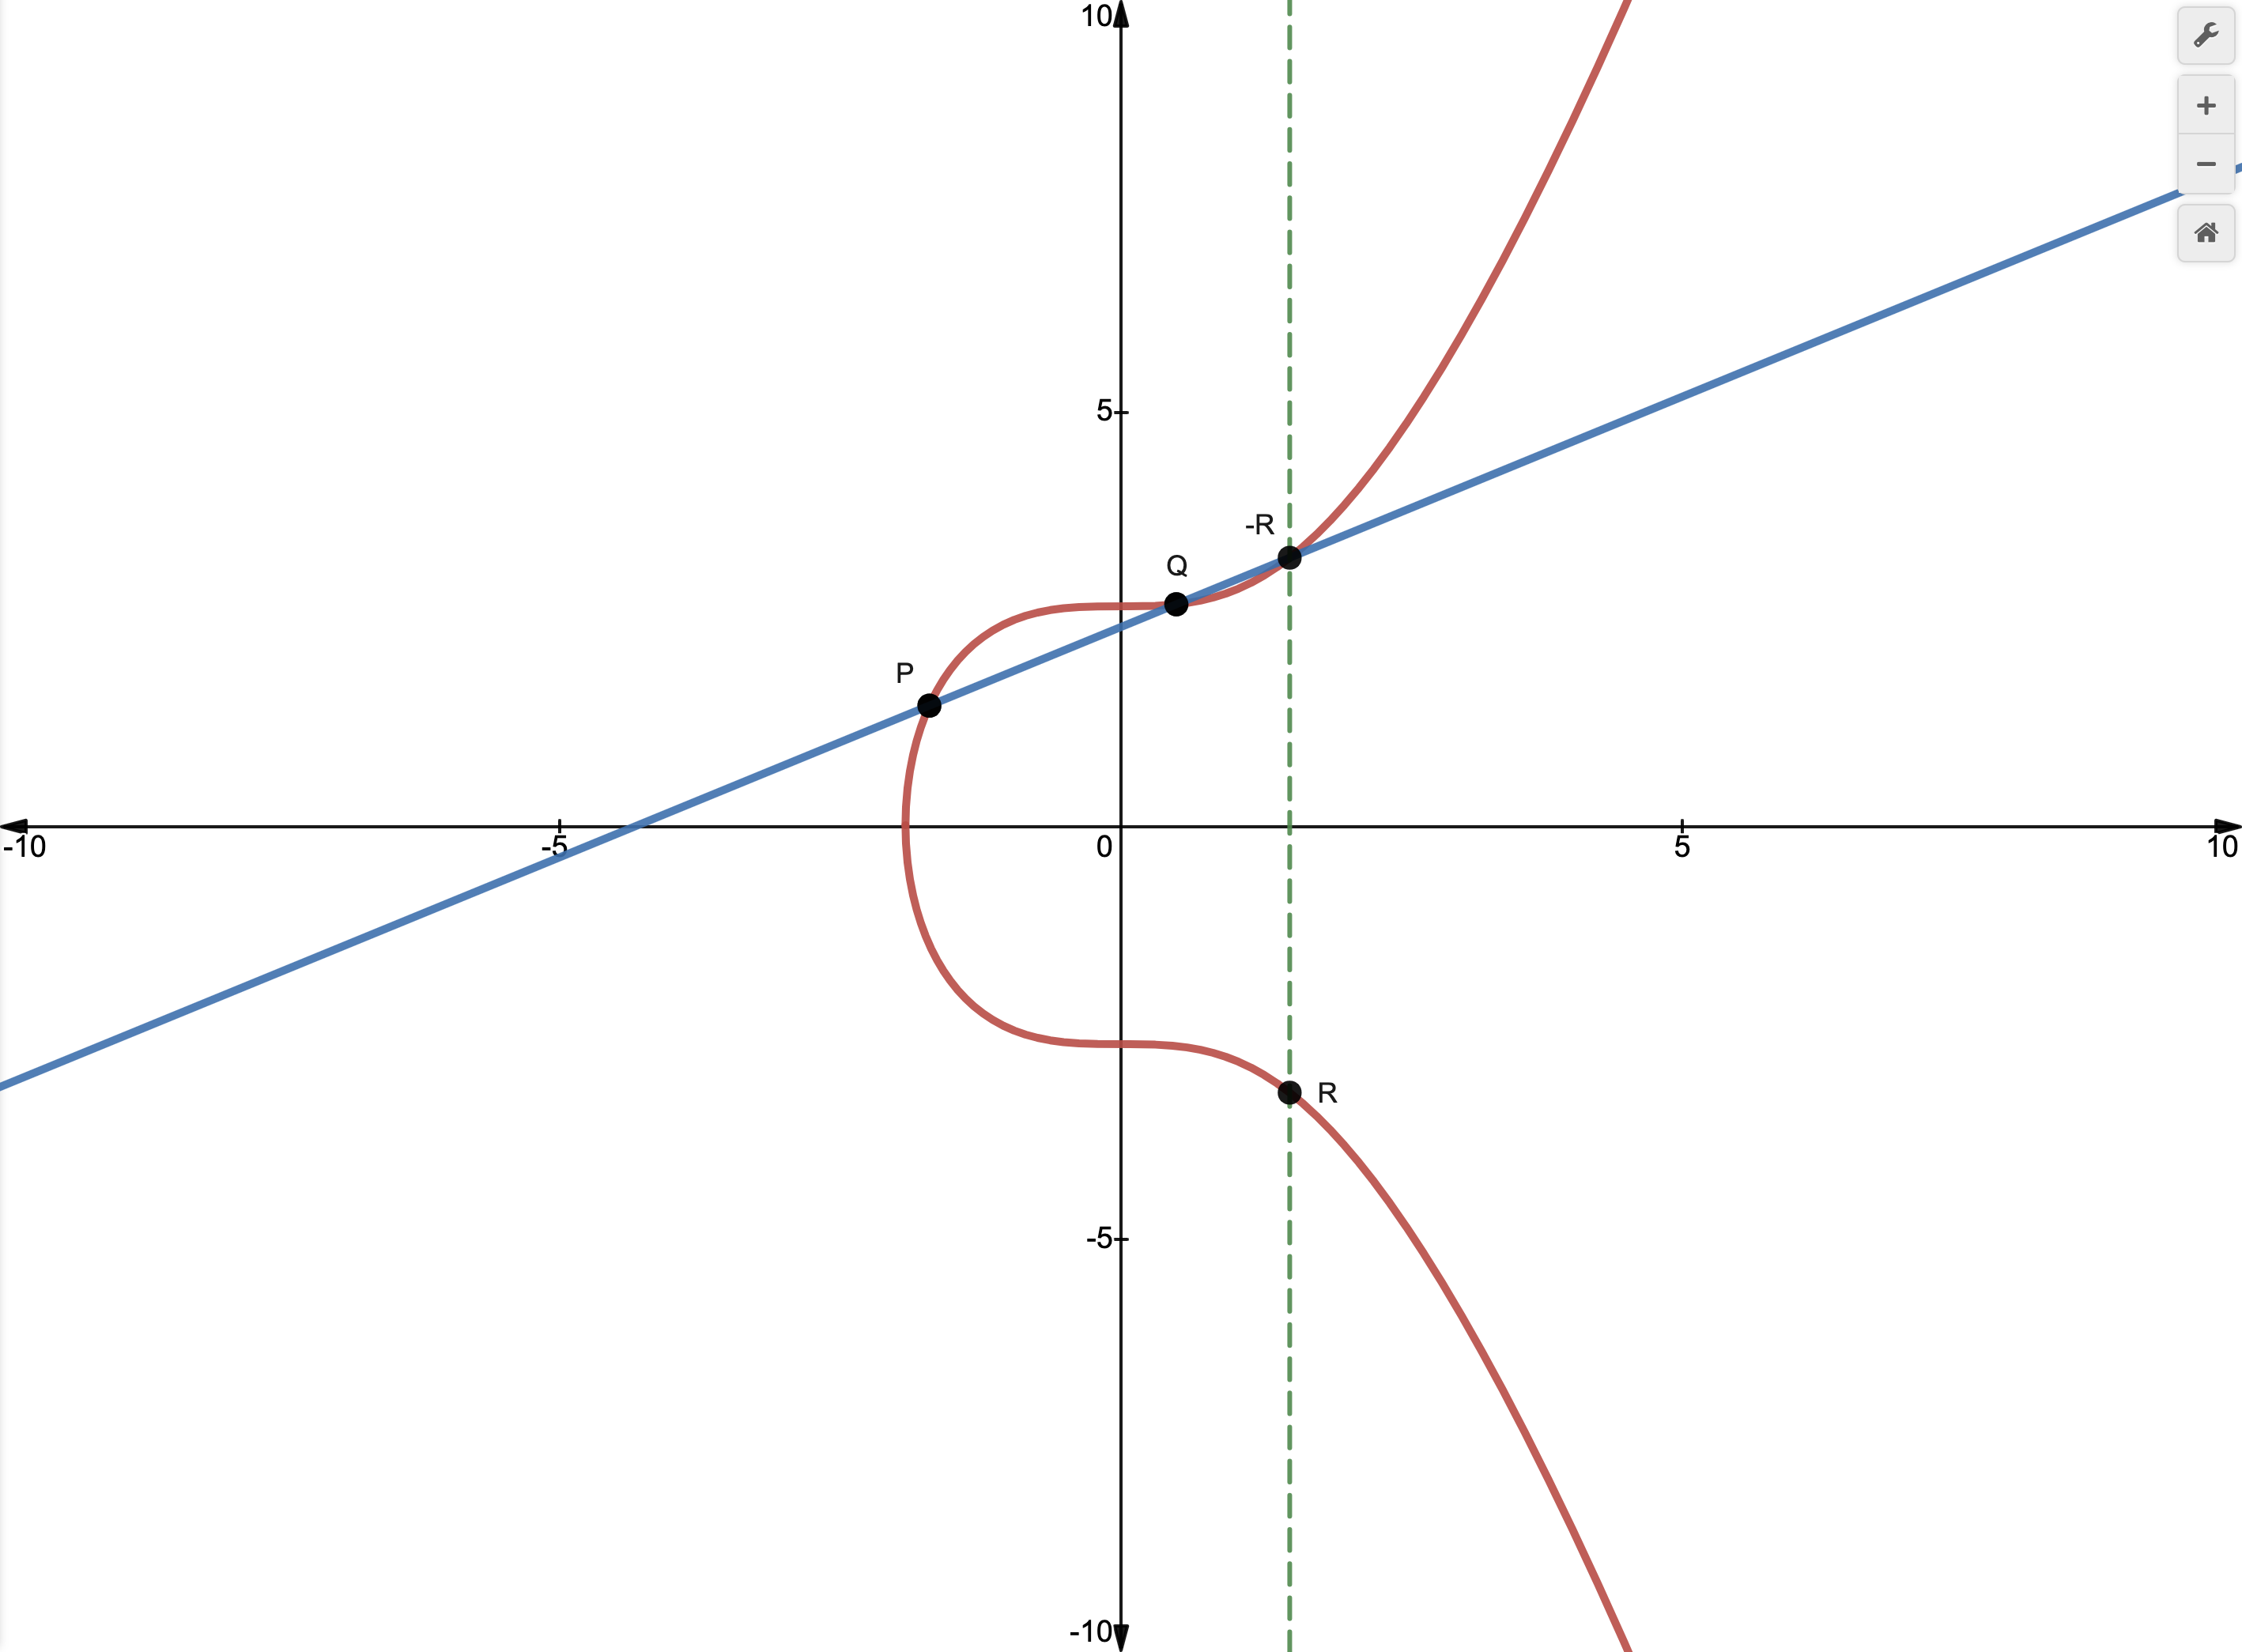
\includegraphics[width=0.5 \textwidth]{images/point_addition.png}
        \caption{\textit{Point addition}}
    \end{center}
\end{figure}

\paragraph{Point doubling}

\tab Point doubling consists of following this steps:

\begin{itemize}
    \item Take a point of the elliptic curve, \(P\).
    \item Pass a tangent line tangent to \(P\).
    \item Mark the point (\(-R\)) from the intersection of the previous line with the curve.
    \item Mirror \(-R\) through the x-axis, obtaining \(R\).
\end{itemize}

This algorithm can be put into the following expression:

\[P + P = 2P = R\]

With \(R\) being the result of the sum of \(R\) with itself.

Finally, this equation can be translated to the following graphic:

\begin{figure}[H]
    \begin{center}
        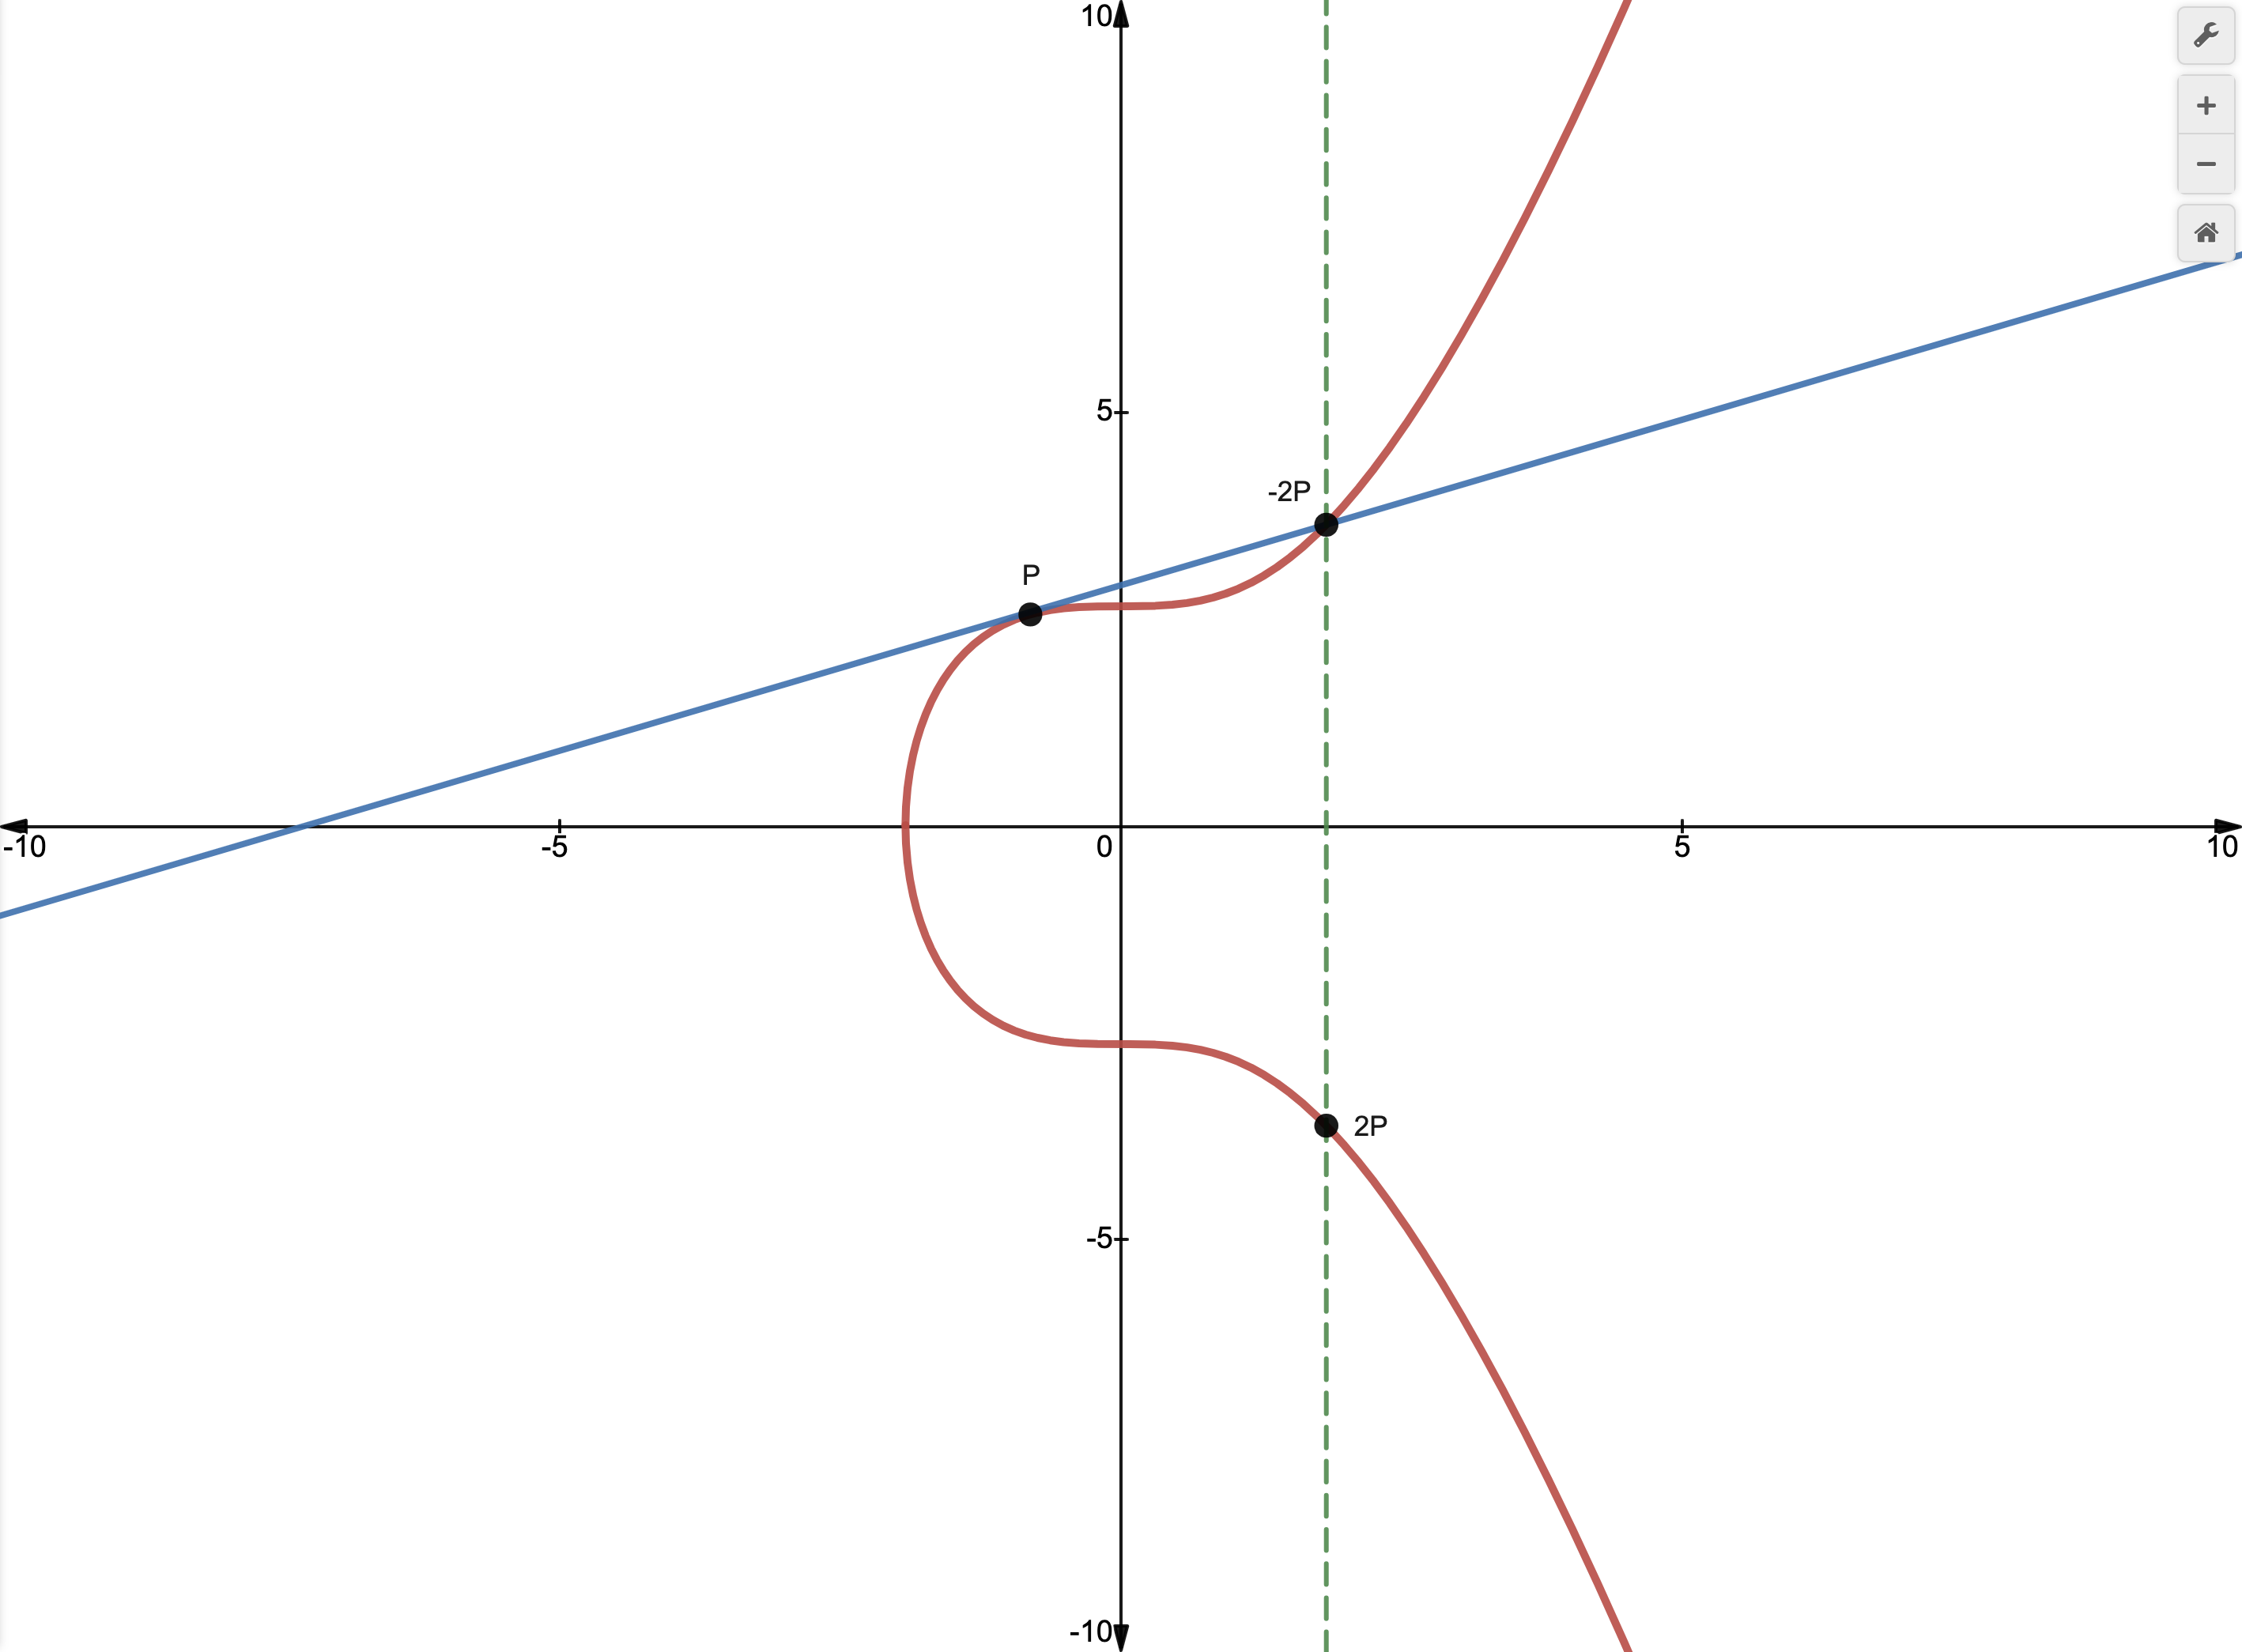
\includegraphics[width=0.5 \textwidth]{images/point_doubling.png}
        \caption{\textit{Point doubling}}
    \end{center}
\end{figure}

\paragraph{Scalar multiplication}

\tab Point addition and point doubling combined are used for scalar multiplication, this means adding a point to itself \(n\) times:

\[R = nP\]

To explain it better, we will use the following example:

\[R = 11P\]
\[R = P + (P + (P + (P + (P + (P + (P + (P + (P + (P + P)))))))))\]

This can be simplified using the previous operations:

\[R = 11P\]
\[R = P + 10P\]
\[R = P + 2(5P)\]
\[R = P + 2(P + 4P)\]
\[R = P + 2(P + 2(2P))\]

As we can see, we just decomposed \(11P\) into two point additions and three point doubling. This can be very useful when \(n\) is a large number.

One of the uses of scalar multiplication is to calculate the private-public key pair, we will take a look on how it works and where it is placed in the Bitcoin protocol in the section bellow.

\subsubsection{Private-Public key pair generation}

\tab The private-public key pair is used on Bitcoin transactions between users. This keys can be represented as:

\begin{itemize}
    \item \textbf{Public key} - represents a public Bitcoin address
    \item \textbf{Private key} - personal key, secret and unique to each user.
\end{itemize}

For generating this pair, we first need a initial point, usually referred as generator point. This point multiplied by the private key will give us the public key:

\[public\: key = generator\: point \times private\: key\]

This is the same as saying that we will add the point to itself as many times as the private key value.

Graphically is easier to understand this. For instance, if we take a point \(P\) of the \textit{secp256k1} curve, and we say that the private key is 4, we will add P to itself 4 times, obtaining \(4P\), this would be the value of the public key associated with the given private one. The process would result in this graph:

\begin{figure}[H]
    \begin{center}
        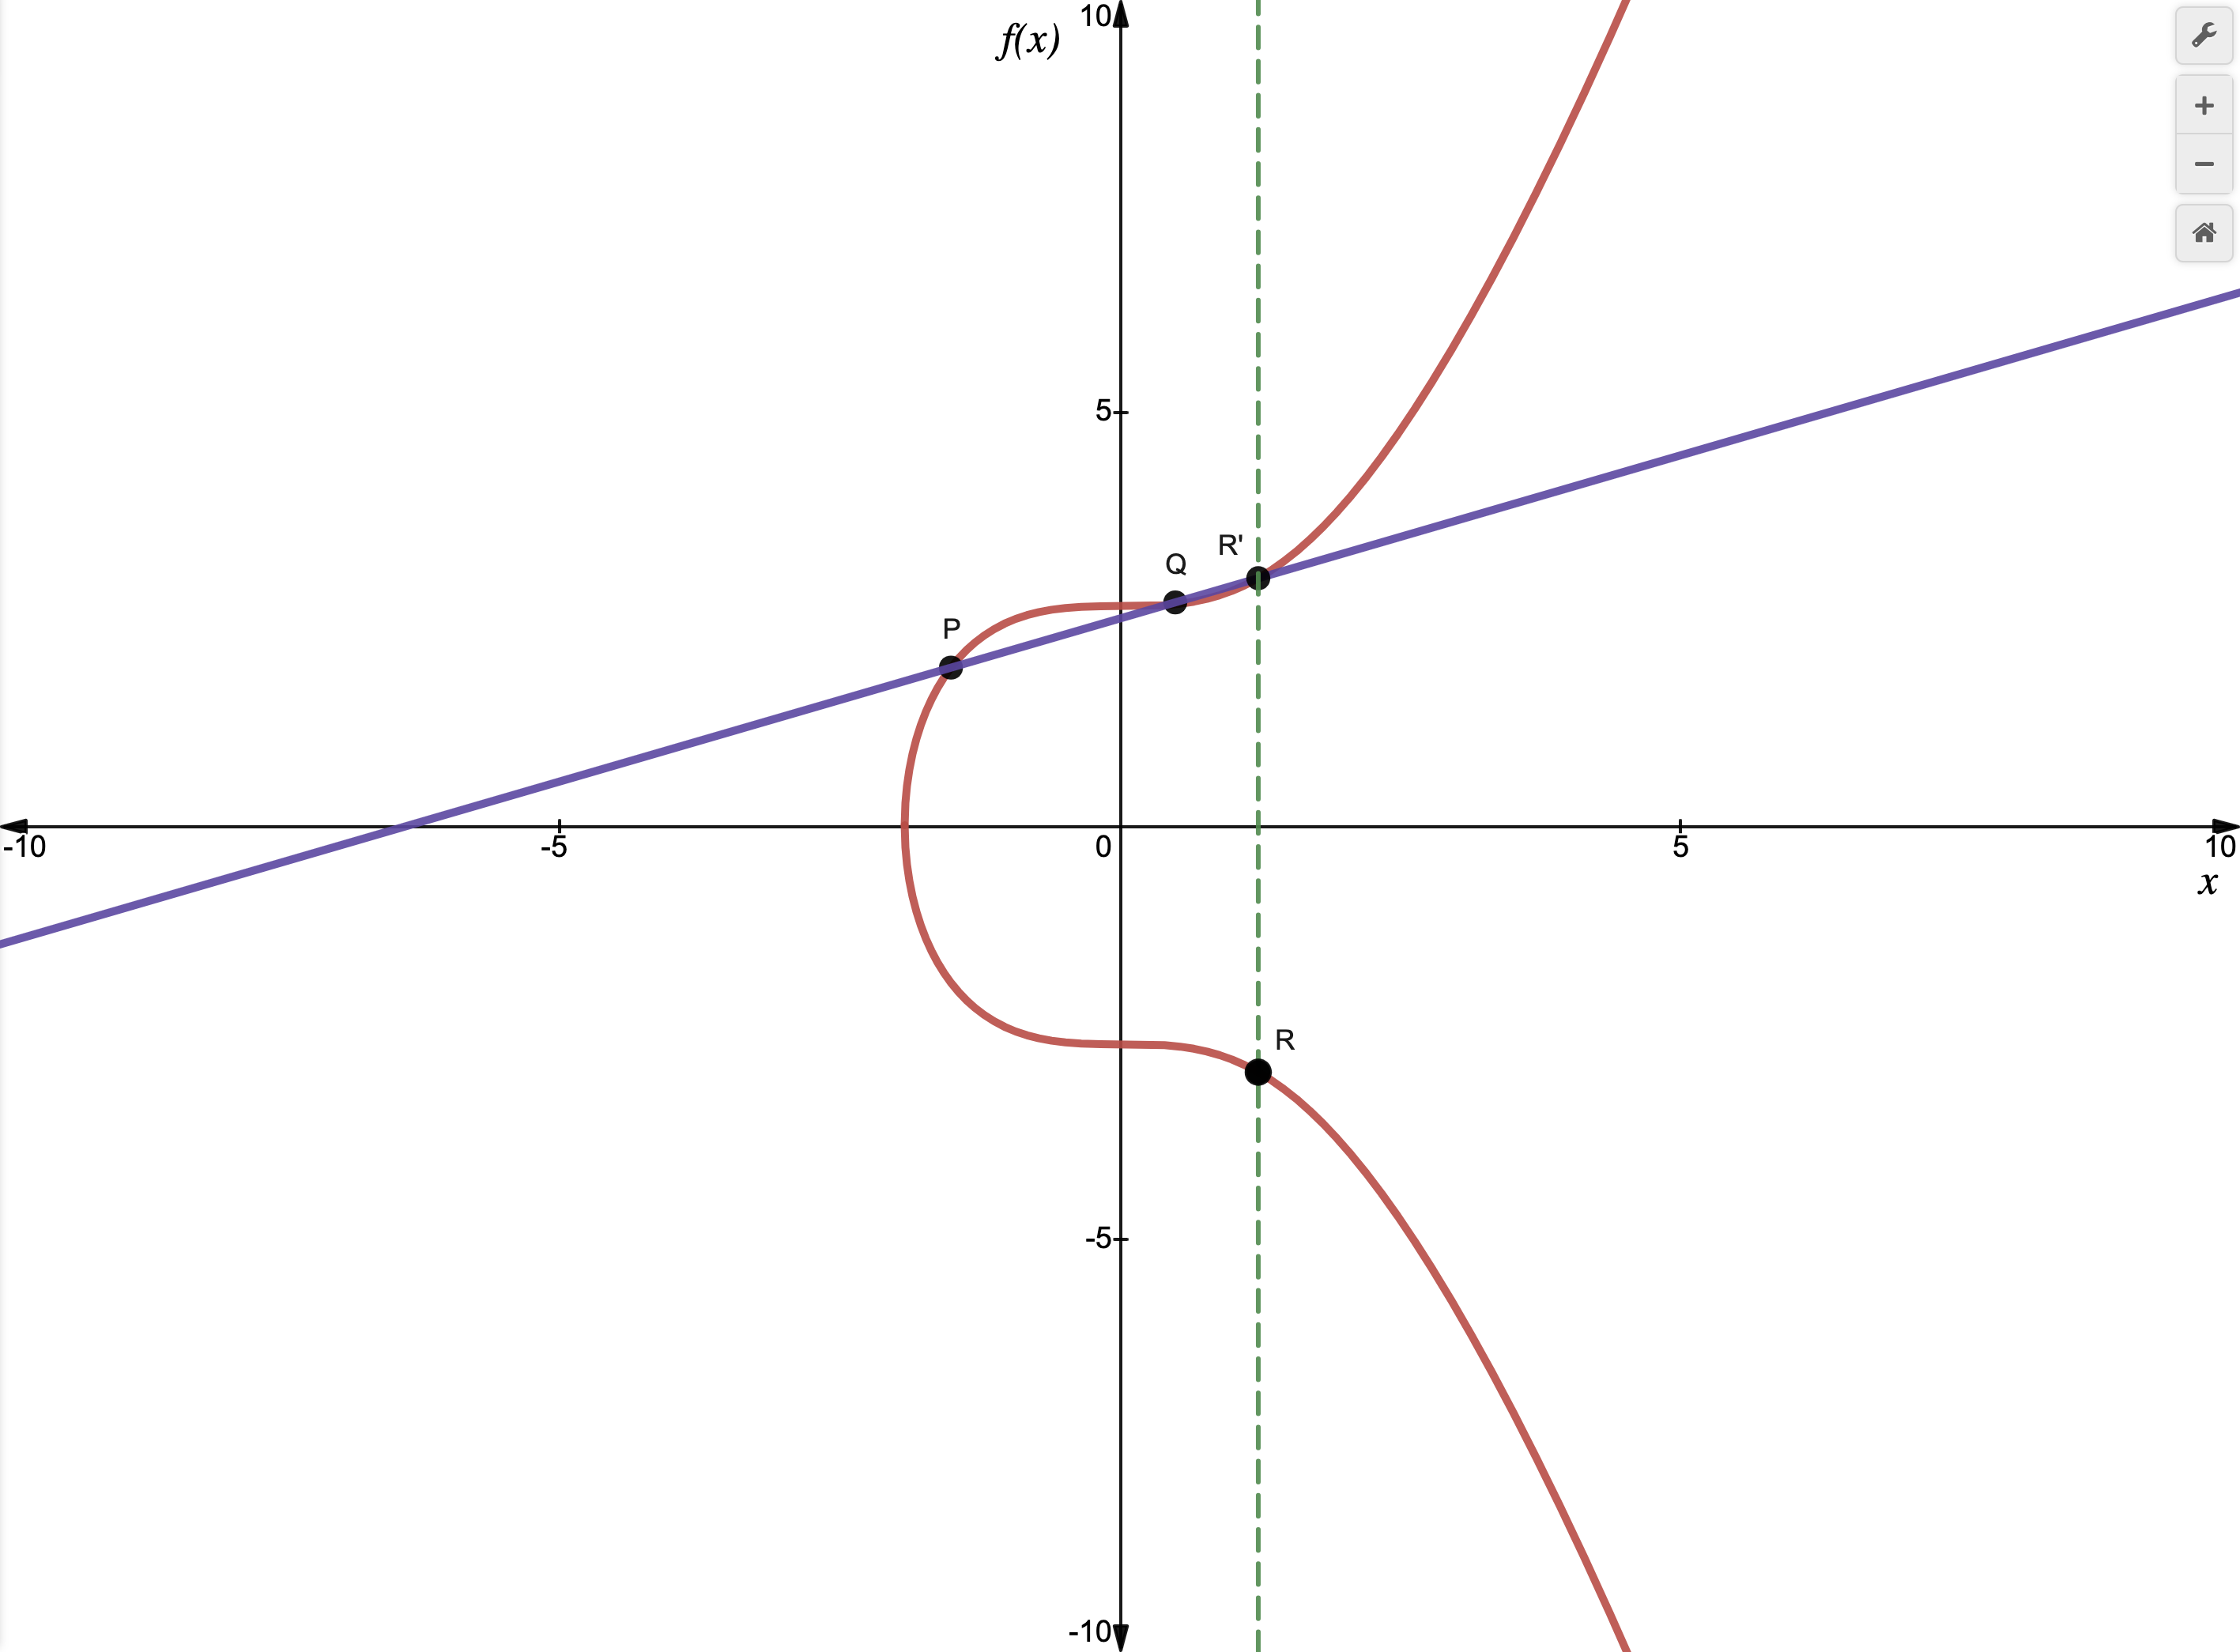
\includegraphics[width=0.5 \textwidth]{images/Kobiltz_curve_with_points.png}
        \caption{\textit{Process of obtaining \(4P\) from the point \(P\), using scalar multiplication}}
    \end{center}
\end{figure}

And this is only for a private key of 4, if the private key is a larger number, there are many more calculations to be made, and many other points created during this process. 

As we previously discussed, the curve used for public-private key generation in the case of Bitcoin has a parameter \(p\), that is the prime order. This number, being a large prime number, prevents the points taking decimal numbers, during the scalar multiplication process, making the curve a collection of dots.

On the graph bellow, we can see a "curve" of finite field with \(b = 7\) and \(p = 37\):

\begin{figure}[H]
    \begin{center}
        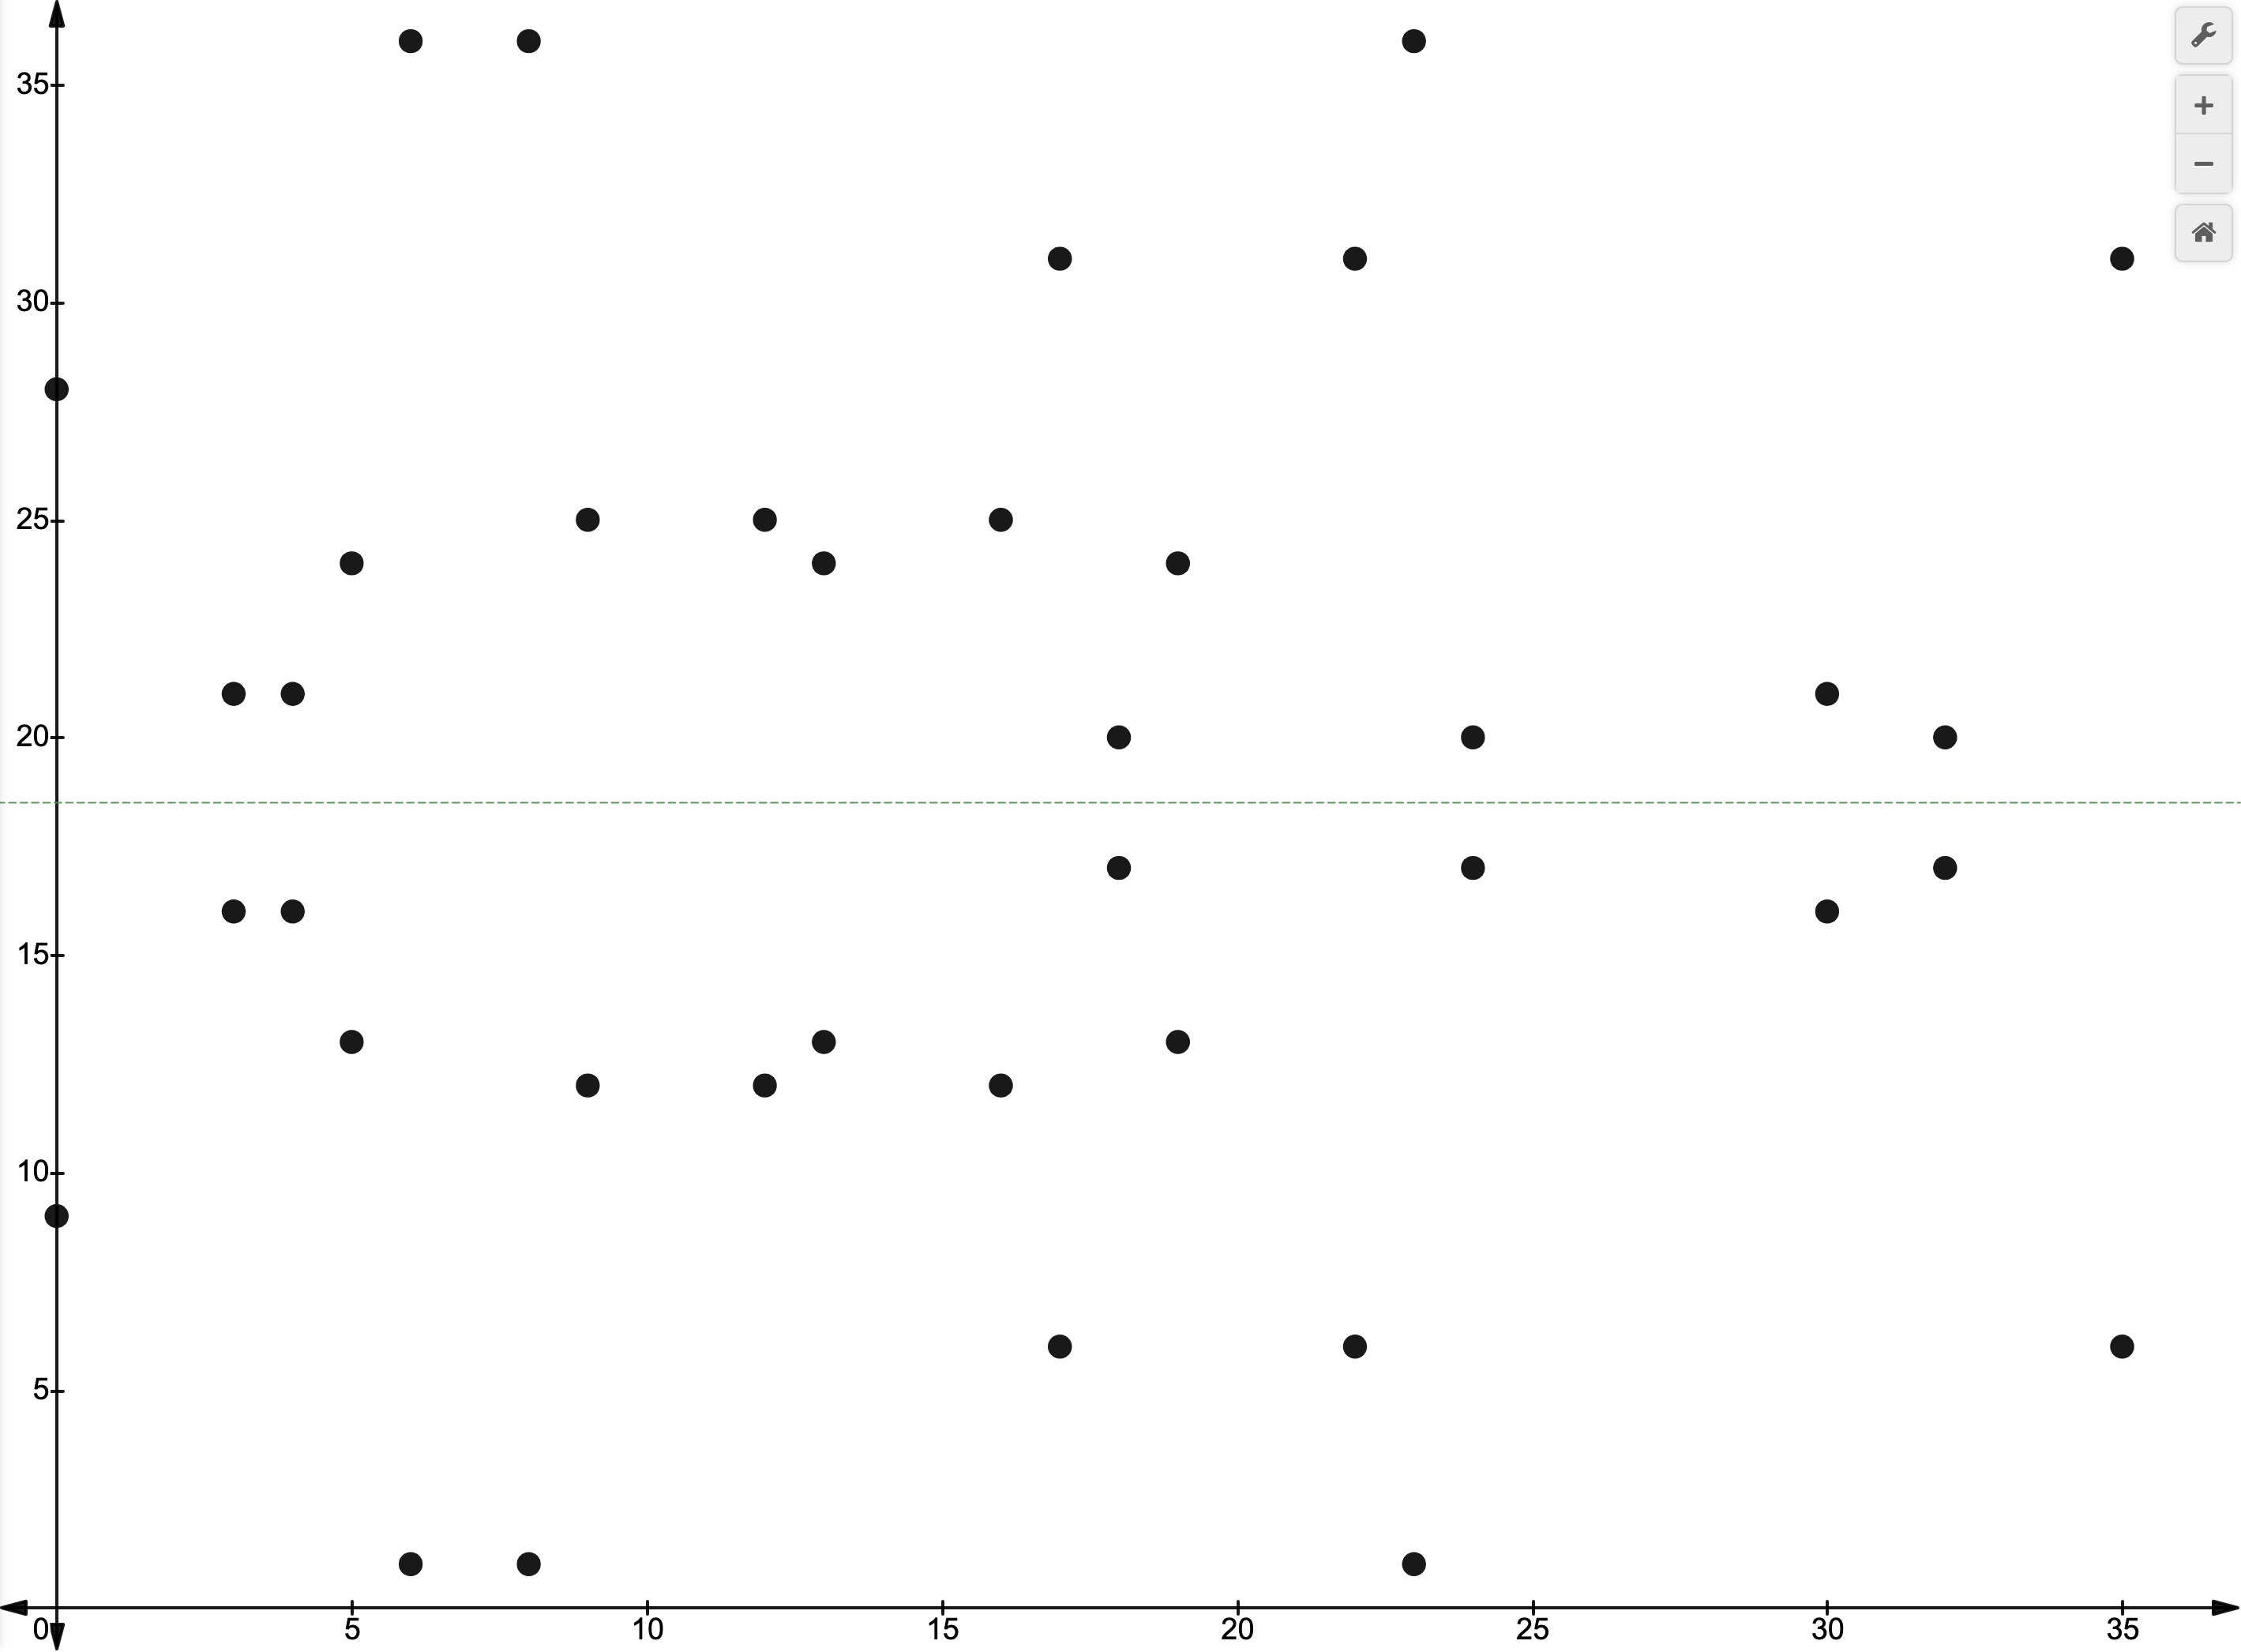
\includegraphics[width=0.6 \textwidth]{images/finite_field_b7_p37.png}
        \caption{\textit{"Curve" of finite field with prime order 37}}
    \end{center}
\end{figure}

Doing this calculation on today's computers is rather fast and efficient, but reversing the same operation is very complex. Although deducing the private key from the public key is possible, it would take a huge time to do so, this process would take \(2^{128}\) attempts, meaning that, even with a million CPU\footnote{Central Processing Unit}s, it would take approximately 260 billion times the age of the universe to break Bitcoin's elliptic curve cryptography.

Generated the pair, this is now used to encrypt data used on Bitcoin transactions.

\section{Socio-Economic Impact of Bitcoin}

\subsection{Price increases and lack of hardware stock related to “Mining”}

\tab GPUs are one of the most important components in a mining Machine as they provide a lot of computational power. GPUs are widely used in many other industries such as the Movie industry, the growing Gaming industry and in the Artificial Intelligence industry. For the mining process to be profitable most miners use more than one GPU on their system (with Warehouses full of them at times) and try to get the more recent versions quickly.

This among other factors creates stock problems in the GPU market as a growing number of miner companies and individual miners take the majority of the stock available and manufacturers can’t keep up with the demand and retailers take advantage and raise the prices as much as three times more than the recommended. (Source: \href{https://videocardz.com/newz/nvidia-geforce-rtx-30-graphics-card-cost-3-times-more-than-nvidia-msrp-in-europe}{VideoCardz})

A side effect of this stock problem is the big impact on the second hand GPU market. With no stock available miners turn to this market and buy everything they can as a Second GPU, performance is  pretty much the same as a brand new one and their slightly reduced life span is not a problem because the goal is always getting the more recent GPU with better performance. Noticing this behavior, second hand sellers took advantage and started to increase prices to a point where some depending on the GPU model that they were selling  would put prices above the retail price.

This made it almost impossible for a normal consumer to get a brand new or used GPU.

In an attempt to correct the situation Manufacturers took some actions. NVIDIA, one of the biggest manufacturers of GPUs, decided to create a dedicated line of GPUs optimized for Professional Mining, the NVIDIA CMP HX. Another critical action taken by NVIDIA to make miners go with the new line optimized for mining was reducing the mining performance of new GPUs produced on the Geforce line, (a line dedicated to Gaming but very appreciated by miners), by reducing the hash rate. 

The effects of these actions in the market is yet to be felt at the time of writing, but many have already criticized NVIDIA because the manufacturer will focus more resources on the professional Mining line of GPUs taking advantage of the growth of mining investors  leaving aside the remaining lines and because this new line of GPUs will have basically no resale value, the GPUs are going to be very disposable and with very little to recycle in this product the environmental impact will increase.

\subsection{Monetary System}

\tab For the time being the impact of Bitcoin on the Monetary systems is close to none as the market capitalisation (814.7 billion U.S. dollars around May 2021) is still small compared with the Market capitalisation of the banking market worldwide (8.9 trillion dollars around the first Q1 of 2021).

To put in another perspective some Central Banks are experimenting with a type of cryptocurrency, but none of the Central Banks plan to use a blockchain based version in their projects, because it was deemed still not mature and stable enough for the infrastructure of national currency to rely on. As Bitcoin relies on blockchain this makes it not suitable and so it does not have a direct impact on the future plans of the Monetary system, because although it does have some big advantages like controlling fraud and maintaining privacy, there are still many cracks that create highways to commit tax evasion or criminal activities.

\subsection{Energy Expenditure}

\tab The mining process of Bitcoin requires machines with a lot of processor power so, consequently, a large energy expenditure is necessary to support the hardware involved in the process like GPUs, which despite major advances in its electrical efficiency still have a significant energy expenditure. Besides energy consumed by more and more machines, individuals and companies with many mining systems or even entire warehouses full of mining systems are investing heavily in refrigeration systems to improve performances and keep the machines constantly working. The energy dispensed in the Mining Process of Bitcoin is commonly known as Bitcoin Energy Consumption and with the growth of the Bitcoin Network this value will consequently increase with time, even with more efficient mining hardware in the future.

If Bitcoin was a country, it would be in the Top 30 energy users worldwide in 2019, according to an analysis made by University of Cambridge. Bitcoin Energy Consumption in 2019 was around 144.28 TWh\footnote{Terawatt-hour}, a value above many developed countries like, Sweden with 131.798 TWh, Netherlands with 110.682 TWh or Portugal with 48.0351 TWh.

\begin{figure}[H]
    \begin{center}
        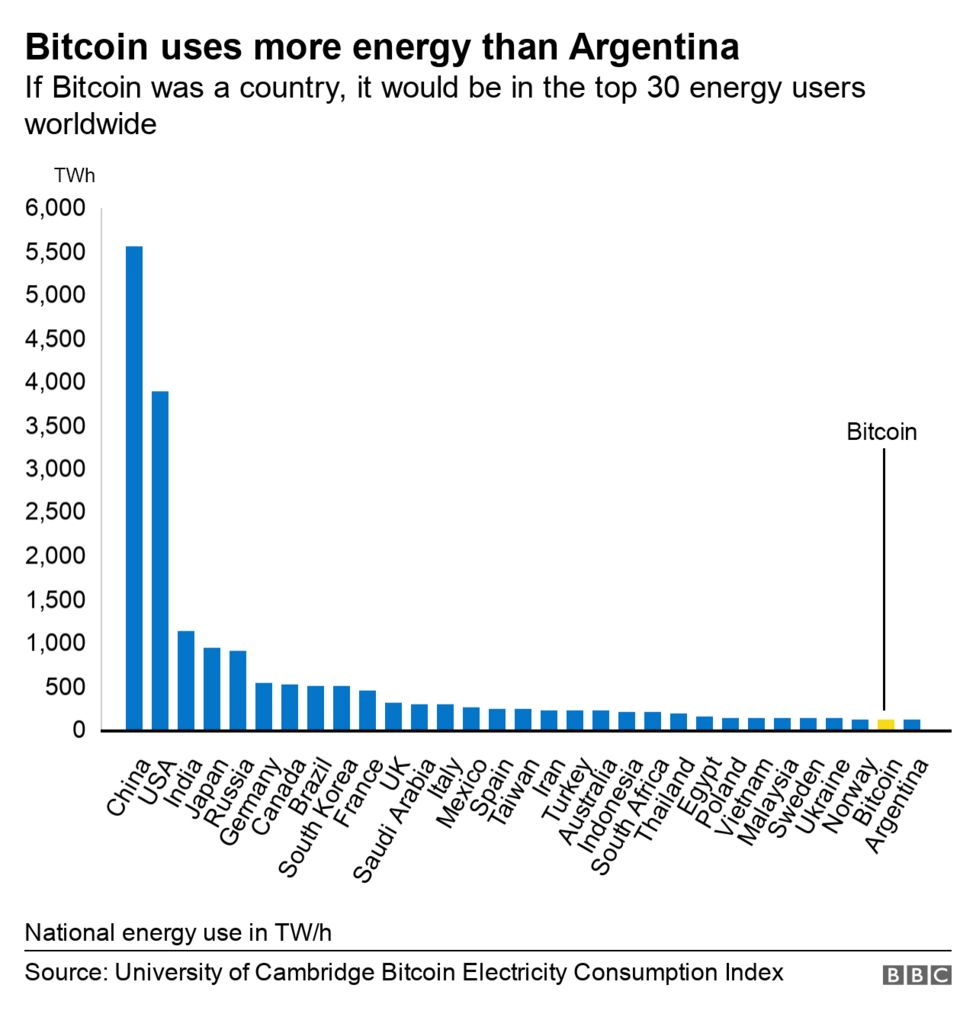
\includegraphics[width=0.6\textwidth]{images/bitcoin_costs.png}
        \caption{\href{https://www.bbc.com/news/technology-56012952}{\underline{Bitcoin’s electricity consumption}}}
    \end{center}
\end{figure}

In order to  get the following results University of Cambridge used a Best-Guess estimate of Bitcoin’s electricity consumption. The method assumes that all miners use an equally-weighted group of hardware types that are profitable in electricity terms, assuming the PUE\footnote{power usage effectiveness} of 1.10. So the Best Guess Power Consumption is calculated by multiplying the average energy efficiency of profitable hardware, with the hashrate, with the PUE with the electricity cost per joule (Pel):

\[E_{estimated}(P_{el}) = \frac{\sum_{i=1}^{N} \vartheta i}{N} * H * PUE * 3.16 * 10^7\]
\[\mbox{with}\]
\[E_{estimated} - \mbox{best guess power consumption (W)}\]
\[\frac{\sum_{i=1}^{N} \vartheta i}{N} - \mbox{average energy efficiency of profitable hardware (J/h)}\]
\[H - \mbox{hashrate (h/s)}\]
\[PUE - \mbox{power usage effectiveness}\]
\[P_{el} - \mbox{electricity cost per joule (USD/J)}\]

The Energy Efficiency of Profitable Hardware, in other words, the Profitability Threshold is calculated by dividing the electricity cost per joule by the mining revenue per hash:

\[\theta = \frac{SRev}{P_{el}}\]
\[\mbox{with}\]
\[\theta - \mbox{profitability threshold (J/h)}\]
\[SRev - \mbox{mining revenue per hash (USD/h)}\]
\[P_{el} - \mbox{electricity cost per joule (USD/J)}\]

This high value of energy consumption comes with many side effects. A  Bitcoin Mining Map from September 2019 to April 2020 created by the University of Cambridge based on geolocation data (i.e. IP addresses) of “hashers” connecting to the Bitcoin mining pools BTC.com, Poolin, and ViaBTC, indicates that from September 2019 to April 2020  roughly 71,70\% of Bitcoin mining was done in China.

\begin{figure}[H]
    \begin{center}
        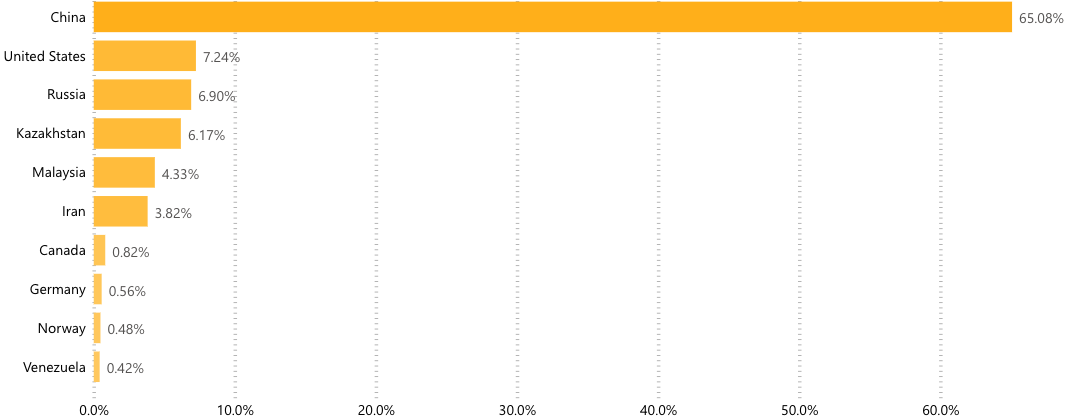
\includegraphics[width=0.8\textwidth]{images/hashrate.png}
        \caption{\href{https://cbeci.org/mining_map}{\underline{Average monthly share of total hashrate}}}
    \end{center}
\end{figure}

This fact is important, because it means that the Bitcoin Network depends heavily on coal-based power that produces some of the worst emissions, which increases Bitcoin's carbon footprint. Many studies have approached  this situation with one study indicating that growth in bitcoin mining alone could result in a 2 degree Celsius increase in global temperatures, although many say such estimates are inflated as miners increasingly go to sources of cheap renewable energy, like hydropower and another study says that bitcoin’s mining carbon footprint in China can threaten its climate change targets.

These discoveries and studies recently made a big negative impact on Bitcoin's reputation as people increasingly understand the effects of climate change and prefer solutions based mostly in green energy to those who don’t. This also led to a statement, on 12 of may, from Tesla's CEO Elon Musk informing that Tesla has suspended vehicle purchases using Bitcoin because of the concerns regarding the rapidly increasing use of fossil fuels for Bitcoin mining and transactions, especially coal. Although believing and trusting the Bitcoin concept, investing in it would go against Tesla’s mission to accelerate the world’s transition to sustainable energy. (Source: https://twitter.com/elonmusk/status/1392602041025843203)

This means that controlling the energy expenditure and transitioning to sustainable energy are some of the challenges for Bitcoin in the next few years.

\subsection{Political implications}

Virtually everything can be used politically and Bitcoin is no exception. Some governments consider Bitcoin a menace because it doesn't have a central authority and that can destabilize or undermine the authority or control of central banks or even from the government itself. Bitcoin anonymity can be used to circumvent capital controls, for money laundering or illegal purchases, and Bitcoin it’s still too risky for many investors, with for example Bitcoin being recently connected to the US Capitol attack where a Large bitcoin payment was made to far-right individuals before the attack.

For that many politicians point out many of the problems surrounding Bitcoin like its energy expenditure, to disrupt people's trust in the cryptocurrency. Other politicians take a different route and prefer to elaborate taxes surrounding Bitcoin gains and transfers to discourage some investors and at same time gain money on taxes, Portugal for example can still be considered a fiscal paradise regarding Bitcoin gains, but many are already proposing taxes and regulation.

Despite this government distrust of Bitcoin and in general from cryptocurrencies, many consider that different cryptocurrencies have different supports with many indicating that Bitcoin is supported by more right-wing and extremist right-wing individuals as explored in the book “The Politics of Bitcoin: Software as Right-wing Extremism", by David Golumbia, while the rival Ethereum is supported by more left wing and extremist left-wing individuals as shown in a survey conducted by CoinDesk with 1200 cryptocurrency users in 2018, found out that 55\% of “Ethereans” tended left ideologies, while 55\% of “Bitcoiners” tended Right ideologies.

\section{Conclusion}

\tab From the analysis and discussion of cryptocurrencies, more specifically Bitcoin, we can infer that, thanks to the advanced technologies and processes that it uses as Blockchain, that allows Bitcoin and most cryptocurrencies to have characteristics very appreciated and valued nowadays, that shows potential to compete with the current monetary system, and in this way, the same already manages to have a sufficient level of support and trust from people in a way that we can’t ignore it anymore and proof of that are the socio-economic effects caused by Bitcoin that are reflected by the whole population regardless of whether or not persons have a direct connection with Bitcoin or with any cryptocurrency.

Despite these levels of trust and support Bitcoin still needs to solve many of its problems, some derived from its special characteristics to have a real, effective, and strong impact on the current monetary system.

\newpage

% Add "References" to table of contents
\addcontentsline{toc}{section}{References}
% No cite makes all references appear, even if there's no citation on the text
\nocite{*}
\printbibliography

\end{document}